%                                                                 aa.dem
% AA vers. 9.1, LaTeX class for Astronomy & Astrophysics
% demonstration file
%                                                       (c) EDP Sciences
%-----------------------------------------------------------------------
%
% \documentclass[referee]{aa} % for a referee version
%\documentclass[onecolumn]{aa} % for a paper on 1 column  
%\documentclass[longauth]{aa} % for the long lists of affiliations 
%\documentclass[letter]{aa} % for the letters 
%\documentclass[bibyear]{aa} % if the references are not structured 
%                              according to the author-year natbib style

%

\documentclass{aa}  

%
\usepackage{graphicx}
\usepackage{amsmath,amsfonts,amssymb}
\usepackage{natbib}
\usepackage{tabularx}
\usepackage{collcell}
\usepackage{array}
\usepackage{booktabs}

%%%%%%%%%%%%%%%%%%%%%%%%%%%%%%%%%%%%%%%%
\usepackage{txfonts}
\usepackage{xcolor}
\usepackage{blindtext}
%%%%%%%%%%%%%%%%%%%%%%%%%%%%%%%%%%%%%%%%
% \usepackage[options]{hyperref}
% To add links in your PDF file, use the package "hyperref"
% with options according to your LaTeX or PDFLaTeX drivers.
\usepackage{float}
%\usepackage{stfloats}
\usepackage{dblfloatfix}
\usepackage{afterpage}
\usepackage{ifthen}
\usepackage[morefloats=12]{morefloats}

\usepackage{placeins}
\usepackage{multicol}
%\usepackage[breaklinks,colorlinks,citecolor=blue]{hyperref}
\bibpunct{(}{)}{;}{a}{}{,}
\usepackage[switch]{lineno}
\definecolor{linkcolor}{rgb}{0.6,0,0}
\definecolor{citecolor}{rgb}{0,0,0.75}
\definecolor{urlcolor}{rgb}{0.12,0.46,0.7}
\usepackage[breaklinks, colorlinks, urlcolor=urlcolor,
linkcolor=linkcolor,citecolor=citecolor,pdfencoding=auto]{hyperref}
\hypersetup{linktocpage}
\usepackage{bold-extra}

%Planck style file, to be used with A&A style to produce Planck papers for publication.
%
% version 28 September 2010 --- useful macros --- CRL
% version 17 October 2010   --- first cut at important instrument values, from Daniele Mennella and
%                               Francois Bouchet, 13 October 2010 --- CRL
% version 18 October 2010   --- LFI FWHM changed to one value per feed, rather than M & S separately
%                               LFI FWHM uncertainties added for individual feeds.  Corrections made
%                               to LFI values. --- Andrea Zacchei
% version 24 October 2010   --- added to and corrected definitions.  No changes made to instrument
%                               quantities. --- CRL 
% version 31 October 2010   --- added definition of \muKHz. --- CRL
%
% version 15 November 2010  --- fixed conflict with aa.cls in definition of \endtable
%                               by naming the command below "\endPlancktable".  See section
%                               13.16 of the Style Guide.
%
% version 06 December 2010  --- Set up names with and without units.
%                               Add \allearlypapers command to ensure that all early papers are
%                               included in the reference list.
%                               Define macro for the name of the 4He JT cooler.
%
% version 07 December 2010  --- removed extraneous "planck2011-1.2" entry in \allearlypapers
%
% version 12 December 2010  --- added \endPlancktablewide command to set tablenotes to the full
%                               page width in the \begin{table*}...\end{table*} environment when
%                               the ``twocolumn'' option is specified in the \documentclass command.
%                               (It would be more elegant to extract the appropriate width from the
%                               aa.cls system at the time of execution, but that is buried more
%                               deeply in the system than I investigated.)
%
% version 05 January 2011   --- added unit \MJysr.  HFI performance values updated per FRB email
%                               01/05/2011 02:38-0800, and Brendan Crill email 01/05/2011 18:08 -0800.
%
% version 06 January 2011   --- changed \scriptscriptstyle primes to \scriptstyle, to better match the
%                               tx fonts used by A&A.
%
% version 07 January 2011   --- modified \allearlypapers to correspond with final early paper list.  
%                               Fixed 545 GHz center frequency.
%
% version 07 January 2011b  --- changed LFI white-noise sensitivity numbers to correct problem with units
%
% version 05 July 2011      --- added \Msol and \Lsol to get the symbols for solar mass and luminosity.
%                               Deleted previous definitions of \solar and \sol, which were equivalent
%                               to the new \Msol.
%
% version 16 August 2011    --- changed comments on \endPlancktable and \endPlancktablewide for clarity
%
% version 11 September 2011 --- changed definition of \tablenote to make footnote labels italic, as per A\&A
%
% version 26 April 2011     --- changed definition of \Planck to agree with what is said in the Style Guide (!)
%
% version 04 Dec 2013       --- included 2013 results references
%
% version 17 Jan 2014       --- included fix to bibtex file v4.3, i.e. \providecommand{\sorthelp}[1]{}
%
% version 26 Jul 2014       --- fixed incompatibility problem with aa.cls v8.0 and v8.2.  v8.2 should now be used
%                               for all Planck papers.
%                           --- fixed problem in definition of "\all2013resultspapers" that introduced a blanck
%                               into the reference to p06b.
%                           --- removed all the parameter definition stuff at the end.  We weren't using it, and
%                               it took up a lot of space.
%
% version 28 Jan 2015       --- added "\alltwentyfiftennresultspapers" and corrected "\all2013resultspapers" to
%                               "\all20thirteenresultspapers",
%
% Usage:  after the \documentclass[traditabstract]{aa} command in the La\TeX\ input file,
%         add this command:      \input Planck.tex


\def\setsymbol#1#2{\expandafter\def\csname #1\endcsname{#2}}
\def\getsymbol#1{\csname #1\endcsname}

%-----------------------------------------------------------------------
% Planck
%-----------------------------------------------------------------------
\def\Planck{\textit{Planck}}

%-----------------------------------------------------------------------
% The Planck Helium-4 JT cooler
%-----------------------------------------------------------------------
\def\HeJT{$^4$He-JT}

%-----------------------------------------------------------------------
% To include all Planck Early Results papers in the reference lists
%-----------------------------------------------------------------------
\def\allearlypapers{\nocite{planck2011-1.1, planck2011-1.3, planck2011-1.4, planck2011-1.5, planck2011-1.6, planck2011-1.7, planck2011-1.10, planck2011-1.10sup, planck2011-5.1a, planck2011-5.1b, planck2011-5.2a, planck2011-5.2b, planck2011-5.2c, planck2011-6.1, planck2011-6.2, planck2011-6.3a, planck2011-6.4a, planck2011-6.4b, planck2011-6.6, planck2011-7.0, planck2011-7.2, planck2011-7.3, planck2011-7.7a, planck2011-7.7b, planck2011-7.12, planck2011-7.13}}

%-----------------------------------------------------------------------
% To include all Planck 2013 Results papers in the reference lists
%-----------------------------------------------------------------------
\def\alltwentythirteenresultspapers{\nocite{planck2013-p01, planck2013-p02, planck2013-p02a, planck2013-p02d, planck2013-p02b, planck2013-p03, planck2013-p03c, planck2013-p03f, planck2013-p03d, planck2013-p03e, planck2013-p01a, planck2013-p06, planck2013-p03a, planck2013-pip88, planck2013-p08, planck2013-p11, planck2013-p12, planck2013-p13, planck2013-p14, planck2013-p15, planck2013-p05b, planck2013-p17, planck2013-p09, planck2013-p09a, planck2013-p20, planck2013-p19, planck2013-pipaberration, planck2013-p05, planck2013-p05a, planck2013-pip56, planck2013-p06b, planck2013-p01a}}

%-----------------------------------------------------------------------
% To include all Planck 2015 Results papers in the reference lists
%-----------------------------------------------------------------------
\def\alltwentyfifteenresultspapers{\nocite{planck2014-a01, planck2014-a03, planck2014-a04, planck2014-a05, planck2014-a06, planck2014-a07, planck2014-a08, planck2014-a09, planck2014-a11, planck2014-a12, planck2014-a13, planck2014-a14, planck2014-a15, planck2014-a16, planck2014-a17, planck2014-a18, planck2014-a19, planck2014-a20, planck2014-a22, planck2014-a24, planck2014-a26, planck2014-a28, planck2014-a29, planck2014-a30, planck2014-a31, planck2014-a35, planck2014-a36, planck2014-a37, planck2014-ES}}

%-----------------------------------------------------------------------
% Tables
%-----------------------------------------------------------------------
\newbox\tablebox    \newdimen\tablewidth
\def\leaderfil{\leaders\hbox to 5pt{\hss.\hss}\hfil}
%
% use the following definition of \endPlancktable for ApJ style notes to tables, set to the 
%         width of the table
% \def\endPlancktable{\tablewidth=\wd\tablebox 
%
% use the following definitions of \endPlancktable and \endPlancktablewide for A&A style notes 
% set to one-column  or full-page width, respectively
\def\endPlancktable{\tablewidth=\columnwidth 
    $$\hss\copy\tablebox\hss$$
    \vskip-\lastskip\vskip -2pt}
\def\endPlancktablewide{\tablewidth=\textwidth 
    $$\hss\copy\tablebox\hss$$
    \vskip-\lastskip\vskip -2pt}
\def\tablenote#1 #2\par{\begingroup \parindent=0.8em
    \abovedisplayshortskip=0pt\belowdisplayshortskip=0pt
    \noindent
    $$\hss\vbox{\hsize\tablewidth \hangindent=\parindent \hangafter=1 \noindent
    \hbox to \parindent{$^#1$\hss}\strut#2\strut\par}\hss$$
    \endgroup}
\def\doubleline{\vskip 3pt\hrule \vskip 1.5pt \hrule \vskip 5pt}

%-----------------------------------------------------------------------
% useful macros
%-----------------------------------------------------------------------
%
\def\L2{\ifmmode L_2\else $L_2$\fi}
%
\def\dtt{\Delta T/T}
\def\DeltaT{\ifmmode \Delta T\else $\Delta T$\fi}
\def\deltat{\ifmmode \Delta t\else $\Delta t$\fi}
\def\fknee{\ifmmode f_{\rm knee}\else $f_{\rm knee}$\fi}
\def\Fmax{\ifmmode F_{\rm max}\else $F_{\rm max}$\fi}
%
\def\solar{\ifmmode{\rm M}_{\mathord\odot}\else${\rm M}_{\mathord\odot}$\fi}
\def\Msolar{\ifmmode{\rm M}_{\mathord\odot}\else${\rm M}_{\mathord\odot}$\fi}
\def\Lsolar{\ifmmode{\rm L}_{\mathord\odot}\else${\rm L}_{\mathord\odot}$\fi}
%
\def\inv{\ifmmode^{-1}\else$^{-1}$\fi}
\def\mo{\ifmmode^{-1}\else$^{-1}$\fi}
\def\sup#1{\ifmmode ^{\rm #1}\else $^{\rm #1}$\fi}
\def\expo#1{\ifmmode \times 10^{#1}\else $\times 10^{#1}$\fi}
%
\def\,{\thinspace}
\def\lsim{\mathrel{\raise .4ex\hbox{\rlap{$<$}\lower 1.2ex\hbox{$\sim$}}}}
\def\gsim{\mathrel{\raise .4ex\hbox{\rlap{$>$}\lower 1.2ex\hbox{$\sim$}}}}
\let\lea=\lsim
\let\gea=\gsim
\def\simprop{\mathrel{\raise .4ex\hbox{\rlap{$\propto$}\lower 1.2ex\hbox{$\sim$}}}}
%
\def\deg{\ifmmode^\circ\else$^\circ$\fi}
\def\pdeg{\ifmmode $\setbox0=\hbox{$^{\circ}$}\rlap{\hskip.11\wd0 .}$^{\circ}
          \else \setbox0=\hbox{$^{\circ}$}\rlap{\hskip.11\wd0 .}$^{\circ}$\fi}
\def\arcs{\ifmmode {^{\scriptstyle\prime\prime}}
          \else $^{\scriptstyle\prime\prime}$\fi}
\def\arcm{\ifmmode {^{\scriptstyle\prime}}
          \else $^{\scriptstyle\prime}$\fi}
\newdimen\sa  \newdimen\sb
\def\parcs{\sa=.07em \sb=.03em
     \ifmmode \hbox{\rlap{.}}^{\scriptstyle\prime\kern -\sb\prime}\hbox{\kern -\sa}
     \else \rlap{.}$^{\scriptstyle\prime\kern -\sb\prime}$\kern -\sa\fi}
\def\parcm{\sa=.08em \sb=.03em
     \ifmmode \hbox{\rlap{.}\kern\sa}^{\scriptstyle\prime}\hbox{\kern-\sb}
     \else \rlap{.}\kern\sa$^{\scriptstyle\prime}$\kern-\sb\fi}
%
\def\ra[#1 #2 #3.#4]{#1\sup{h}#2\sup{m}#3\sup{s}\llap.#4}
\def\dec[#1 #2 #3.#4]{#1\deg#2\arcm#3\arcs\llap.#4}
\def\deco[#1 #2 #3]{#1\deg#2\arcm#3\arcs}
\def\rra[#1 #2]{#1\sup{h}#2\sup{m}}
%
\def\page{\vfill\eject}
\def\dots{\relax\ifmmode \ldots\else $\ldots$\fi}
%
%-----------------------------------------------------------------------
% units
%-----------------------------------------------------------------------
%
\def\WHzsr{\ifmmode $W\,Hz\mo\,sr\mo$\else W\,Hz\mo\,sr\mo\fi}
\def\mHz{\ifmmode $\,mHz$\else \,mHz\fi}
\def\GHz{\ifmmode $\,GHz$\else \,GHz\fi}
\def\mKs{\ifmmode $\,mK\,s$^{1/2}\else \,mK\,s$^{1/2}$\fi}
\def\muKs{\ifmmode \,\mu$K\,s$^{1/2}\else \,$\mu$K\,s$^{1/2}$\fi}
\def\muKRJs{\ifmmode \,\mu$K$_{\rm RJ}$\,s$^{1/2}\else \,$\mu$K$_{\rm RJ}$\,s$^{1/2}$\fi}
\def\muKHz{\ifmmode \,\mu$K\,Hz$^{-1/2}\else \,$\mu$K\,Hz$^{-1/2}$\fi}
\def\MJysr{\ifmmode \,$MJy\,sr\mo$\else \,MJy\,sr\mo\fi}
\def\MJysrmK{\ifmmode \,$MJy\,sr\mo$\,mK$_{\rm CMB}\mo\else \,MJy\,sr\mo\,mK$_{\rm CMB}\mo$\fi}
\def\microns{\ifmmode \,\mu$m$\else \,$\mu$m\fi}
\def\micron{\microns}
\def\muK{\ifmmode \,\mu$K$\else \,$\mu$\hbox{K}\fi}
\def\microK{\ifmmode \,\mu$K$\else \,$\mu$\hbox{K}\fi}
\def\muW{\ifmmode \,\mu$W$\else \,$\mu$\hbox{W}\fi}
\def\kms{\ifmmode $\,km\,s$^{-1}\else \,km\,s$^{-1}$\fi}
\def\kmsMpc{\ifmmode $\,\kms\,Mpc\mo$\else \,\kms\,Mpc\mo\fi}
%
%
%----------------------------------------------------------------------
% set up machinery to list Planck papers in roman numeral order.
%----------------------------------------------------------------------

\providecommand{\sorthelp}[1]{}


% Custom definitions
\def\Cosmoglobe{\textsc{Cosmoglobe}}
\def\cosmoglobe{\textsc{Cosmoglobe}}
\def\Planck{\textit{Planck}}


% \renewcommand{\topfraction}{1.0}	% max fraction of floats at top
%     \renewcommand{\bottomfraction}{1.0}	% max fraction of floats at bottom
%     %   Parameters for TEXT pages (not float pages):
%     \setcounter{topnumber}{2}
%     \setcounter{bottomnumber}{2}
%     \setcounter{totalnumber}{4}     % 2 may work better
%     \setcounter{dbltopnumber}{2}    % for 2-column pages
%     \renewcommand{\dbltopfraction}{0.9}	% fit big float above 2-col. text
%     \renewcommand{\textfraction}{0.04}	% allow minimal text w. figs
%     %   Parameters for FLOAT pages (not text pages):
%     \renewcommand{\floatpagefraction}{0.9}	% require fuller float pages
% 	% N.B.: floatpagefraction MUST be less than topfraction !!
%     \renewcommand{\dblfloatpagefraction}{0.9}	% require fuller float pages



\begin{document} 

   \title{\bfseries{\Cosmoglobe\ DR2. II. Bayesian global modelling of zodiacal light\\ with a first application to \textit{COBE}-DIRBE}}

   %This author list corresponds to \title{Author list for L04\_CMB\_Foregrounds\_Extraction}
%Prepared by M. Lopez-Caniego (Marcos.Lopez.Caniego@sciops.esa.int), ESAC/ESA
%This version is from Thu Jul 12 18:11:48 2018 CET
%\subtitle{There are 152 co-authors in this list}
\newcommand{\oslo}[0]{1}
\newcommand{\iiabangalore}[0]{2}

\author{\small
D.~J.~Watts\inst{\ref{uio}}\thanks{Corresponding author: D.~J.~Watts; \url{duncanwa@astro.uio.no}}
\and
A.~Basyrov\inst{\ref{uio}}
\and
H.~T.~Ihle\inst{\ref{uio}}
\and
S.~Paradiso\inst{\ref{waterloo}}
\and
F.~Rahman\inst{\ref{iiabangalore}}
\and
H.~Thommesen\inst{\ref{uio}}
\and
M.~Bersanelli\inst{\ref{milan}}
\and
L.~A.~Bianchi\inst{\ref{milan}}
\and
M.~Brilenkov\inst{\ref{uio}}
\and
L.~P.~L.~Colombo\inst{\ref{milan}}
\and
H.~K.~Eriksen\inst{\ref{uio}}
\and
J.~R.~Eskilt\inst{\ref{uio},\ref{imperial}}
\and
K.~S.~F.~Fornazier\inst{\ref{saopaulo}}
\and
C.~Franceschet\inst{\ref{milan}}
\and
U.~Fuskeland\inst{\ref{uio}}
\and
M.~Galloway\inst{\ref{uio}}
\and
E.~Gjerl\o w\inst{\ref{uio}}
\and
B.~Hensley\inst{\ref{princeton}}
\and
L.~T.~Hergt\inst{\ref{ubc}}
\and
D.~Herman\inst{\ref{uio}}
\and
G.~A.~Hoerning\inst{\ref{saopaulo}}
\and
K.~Lee\inst{\ref{uio}}
\and
J.~G.~S.~Lunde\inst{\ref{uio}}
\and
A.~Marins\inst{\ref{saopaulo},\ref{ustofc}}
\and
S.~K.~Nerval\inst{\ref{dunlap1},\ref{dunlap2}}
\and
S.~K.~Patel\inst{\ref{iit_bhu}}
\and
M.~Regnier\inst{\ref{apc}}
\and
M.~San\inst{\ref{uio}}
\and
S.~Sanyal\inst{\ref{iit_bhu}}
\and
N.-O.~Stutzer\inst{\ref{uio}}
\and
A.~Verma\inst{\ref{iit_bhu}}
\and
I.~K.~Wehus\inst{\ref{uio}}
\and
Y.~Zhou\inst{\ref{berkeley}}
}
\institute{\small
Institute of Theoretical Astrophysics, University of Oslo, Blindern, Oslo, Norway\label{uio}
\and
Waterloo Centre for Astrophysics, University of Waterloo, Waterloo, ON N2L 3G1, Canada\label{waterloo}
\and
Indian Institute of Astrophysics, Koramangala II Block, Bangalore, 560034, India\label{iiabangalore}
\and
Dipartimento di Fisica, Università degli Studi di Milano, Via Celoria, 16, Milano, Italy\label{milan}
\and
Imperial Centre for Inference and Cosmology, Department of Physics, Imperial College London, Blackett Laboratory, Prince Consort Road, London SW7 2AZ, United Kingdom\label{imperial}
\and
Instituto de Física, Universidade de São Paulo - C.P. 66318, CEP: 05315-970, São Paulo, Brazil\label{saopaulo}
\and
Department of Astrophysical Sciences, Princeton University, 4 Ivy Lane, Princeton, NJ 08540\label{princeton}
\and
Department of Physics and Astronomy, University of British Columbia, 6224 Agricultural Road, Vancouver BC, V6T1Z1, Canada\label{ubc}
\and
Department of Astronomy,  University of Science and Technology of China, Hefei, China\label{ustofc}
\and
David A. Dunlap Department of Astronomy \& Astrophysics, University of Toronto, 50 St. George Street, Toronto, ON M5S 3H4, Canada\label{dunlap1}
\and
Dunlap Institute for Astronomy \& Astrophysics, University of Toronto, 50 St. George Street, Toronto, ON M5S 3H4, Canada\label{dunlap2}
\and
Department of Physics, Indian Institute of Technology (BHU), Varanasi - 221005, India\label{iit_bhu}
\and
Laboratoire Astroparticule et Cosmologie (APC), Université Paris-Cité, Paris, France\label{apc}
\and
Department of Physics, UC Berkeley\label{berkeley}
}

 %\author{V.~Arsenijevic\inst{\ref{inst1}}\and S.~Fabbro\inst{\ref{inst2}}\and
%A.~M.~Mour\~ao\inst{\ref{inst3}}\and A.~J.~Rica da Silva\inst{\ref{inst1}}}
%
%\institute{Multidisciplinar de Astrof\'{\i}sica, IST, Avenida Rovisco Pais, 1049
%Lisbon, Portugal\email{...}\label{inst1} \and < Multidisciplinar de Astrof\'{\i}sica, IST, Avenida Rovisco Pais, 1049 Lisbon, Portugal\email{...}\label{inst2}
%\and
%Multidisciplinar de Astrof\'{\i}sica, IST, Avenida Rovisco Pais, 1049
%Lisbon, Portugal\email{...}\label{inst3}
%} 


   \institute{Institute of Theoretical Astrophysics, University of Oslo, Blindern, Oslo, Norway}
  
   % Shortened title, author list for top of page 
   \titlerunning{\Cosmoglobe: Interplanetary dust}
   \authorrunning{M.~San et al.}

   \date{\today}
   

% write an abstract 

\abstract{We present the first Bayesian framework for global modelling of zodiacal light and its application to the Diffuse Infrared Background Experiment (DIRBE) time-ordered data (TOD). The framework uses a modified version of the COBE/DIRBE zodiacal light model to estimate the zodiacal light along the observed line-of-sights in the time domain. We obtain a new state-of-the-art zodiacal light model by re-estimating the free parameters in the COBE/DIRBE model and produce DIRBE zodiacal light subtracted mission average (ZSMA) maps with much smaller zodiacal light residuals. We argue that the improved zodiacal light model fit becomes possible through global Bayesian end-to-end analysis of the DIRBE TODs with COBE-FIRAS, GAIA, Planck HFI, and WISE observations, giving us a more accurate instrumental and astophysical characterization of the infrared sky.
However, we do note that even though the zodiacal light model represent an improvement with respect to original DIRBE model when it comes to removing ZL from the DIRBE data, this is still a preliminary model. We illustrate the potential of this framework for building zodiacal models by conducting a small study where we further extend and modifcations to the zodiacal light model by adding more asteroidal bands, interstellar dust and using a more physically motivated parameterization of the interplanetary medium as described in \cite{RRM}. A more modern and physical parametrization of the interplanetary medium in combination with joint analysis with complementry infrared experiments such IRAS, AKARI, WISE and SPHEREx will 

}

%   \abstract{We present a new and improved interplanetary dust model. The interplanetary dust model is a re-estimation of the parameters in the Kelsall et al. (1998) model in addition to an interstellar dust component inspired by Robinson and May (200?). In addition, other small improvements such as using modern solar irradiance models are included. The model parameters are re-estimated using Commander, where we have added zodiacal parameters as an additional gibbs step. The 180 total parameters in the model are estimated using Gibbs sampling. We demonstrate the use of the new interplanetary model on the binned DIRBE CIOs along with the \Cosmoglobe\ sky model to produce the cleanest to date DIRBE sky maps. The Cosmoglobe model which is valid between 1.25 $\mu m$ and 240 $\mu m$ is added added as the new default interplanetary dust model in ZodiPy.}

   \keywords{Zodiacal dust, Interplanetary medium, Cosmology: cosmic background radiation}

   \maketitle

\setcounter{tocdepth}{3}
%\tableofcontents
   
\section{Introduction}
Zodiacal light (ZL, sometimes zodiacal emission or interplanetary dust emission) is the primary source of diffuse radiation observed in the infrared sky between 1-100 $\mu$m (\cite{Leinert1998} and references therein). The light comes from scattering and re-emission of sunlight from interplanetary dust (IPD) grains. The inner Solar system is embedded in a sun-centered cloud of IPD, with a symmetry axis tilted slightly with respect to the Ecliptic, known as the zodiacal cloud. The ZL is seasonal, and its appearance in the sky changes as the Earth moves through the IPD distribution. The most common way to model the observer position-dependent ZL is to evaluate a line-of-sight integral for each observation directly in the time-ordered domain. The time-varying and three-dimensional nature of the ZL makes it one of the most challenging foregrounds to model in astrophysical and cosmological studies of the infrared sky. The lack of a good ZL model has left a vast portion of the electromagnetic spectrum inaccessible to cosmological analysis attempting to measure the Cosmic Optical and Infrared Backgrounds (COB, CIB). 

The state-of-the-art ZL model in the field of cosmology is the \cite{Kelsall1998} model (K98, sometimes referred to as the \textit{COBE}/DIRBE or just the DIRBE model). K98 is a parametric ZL model describing the three-dimensional IPD distribution and the radiative properties of the dust. The model was developed by the \textit{COBE}/DIRBE team to remove ZL from their data in the late 1900s. Since then, our understanding of the infrared sky has improved with new observational data from experiments like Planck HFI, GAIA, and WISE. Combining recent computational advances in Bayesian cosmological analysis \citep{BP2023, Galloway2023, Watts2023}, more readily available computing power and new complementary infrared datasets allow us to extract significantly more information about the true nature of the ZL from the DIRBE data than was possible at the time of the original DIRBE analysis.

This paper is the second in a series of six describing the methods and results of our re-analysis of the time-ordered \textit{COBE}/DIRBE data within a global end-to-end Bayesian analysis framework. Here, we describe the ZL modeling approach in Commander3 and demonstrate the benefits of fitting a ZL model directly within a global end-to-end Bayesian framework. The basis of the newly implemented ZL module in Commander3 is ZodiPy \citep{San2024}, which is an Astropy-affiliated Python package for ZL simulations. The development of ZodiPy was motivated by two factors. It would serve as a basis for the code development in Commander3, and secondly, it would provide the astrophysical and cosmology communities with an accessible, easy-to-use interface to existing and coming ZL models. As an early application, \cite{San2022} demonstrates the removal of ZL from the DIRBE TOD with ZodiPy using the K98 model.

The following sections are organized as follows. In Sect. \ref{sect:zodi-model}, we introduce the K98 ZL model and discuss implementation details and some optimizations regarding evaluating ZL models on HEALPix grids. Next, in Sect. \ref{sect:param-estimation}, we discuss ZL parameter estimation and our implementation, which involves the use of a function minimizer on a sub-sample of the DIRBE TOD. Finally, in Sect. \ref{sect:improved-model}, we present a greatly improved ZL model, yielding lower residuals at all ten DIRBE channels. The improved model uses only a slightly different parametrization than the K98 model. We recommend using this model over K98 for all infrared community members.

\section{Zodiacal light modelling}\label{sect:zodi-model}
ZL is commonly removed directly from timestreams by performing line-of-sight integration at each observation through a parametric three-dimensional model of the IPD distribution. We use a slightly modified version of the K98 ZL model in Commander3. Below we present a short introduction to the model parametrization in terms of the three-dimensional IPD distribution and the radiative and scattering properties of the IPD. We refer to \cite{Kelsall1998} for a more detailed discussion about the ZL model.
\subsection{Parameterization of interplanetary dust}
The IPD in the zodiacal cloud is smooth and stable, and most of the dust is accounted for by a diffuse cloud-like component \citep{Leinert1998}. The majority of the dust in this cloud component stems from the mass-shedding of Jupiter family comets with low eccentricities and inclinations with respect to the ecliptic. However, fine structures within the zodiacal cloud exist as a result of collisions and fragmentation in asteroids and gravitational resonance in the orbit of planets \citep{Low1984, Dermott1984, Dermott1994, Reach1997}. 

We model the IPD distribution as a combination of several zodiacal components, denoted by $c$, each described by a heliocentric ecliptic number density $n_c(x,y,z)$. Each zodiacal component is allowed to have a heliocentric offset $(x_{0,c}, y_{0,c}, z_{0,c})$, such that the component-centric coordinates become
\begin{equation}    
    \begin{aligned}
        x_c&= x - x_{0,c}\\
        y_c&= y - y_{0,c}\\
        z_c&= z - z_{0,c}.
    \end{aligned}
\end{equation}
Additionally, each zodiacal component is allowed to have a plane of symmetry different from the ecliptic, given by an inclination $i_c$ and ascending node $\Omega_c$. In component-centric coordinates, the number density is then fully described by the radial distance $r_c$ from the origin and the height above the symmetry plane $Z_c$
\begin{align}
    r_c &= \sqrt{x_c^2 + y_c^2 + z_c^2},\\
    Z_c &= x_c\sin{\Omega_c}\sin{i_c} - y_c \cos{\Omega_c}\sin{i_c} + z_c \cos{i_c}.
\end{align}


\subsection{Zodiacal components}
\subsubsection{Smooth cloud}
The cloud component represents the smooth IPD distribution that embeds the inner Solar system. Its number density is modeled as
\begin{equation}
    n_\mathrm{C}(x,y,z)=n_{0, \mathrm{C}}r_\mathrm{C}^{-\alpha}f(\zeta_\mathrm{C}),
\end{equation}
where $n_{0, \mathrm{C}}$ is the number density at 1 AU, $\alpha$ is a power-law index, $f(\zeta_\mathrm{C})$ is the fan-like vertical distribution given as $f(\zeta_\mathrm{C}) = \exp {\left[-\beta g^\gamma \right]}$, where $\zeta_\mathrm{c} = |Z_\mathrm{c}|/r_\mathrm{c}$ is the radial height above the symmetry plane, 
\begin{equation}
    g = \begin{cases}
        \zeta^2/2\mu & \mathrm{for}\; \zeta < \mu,\\
        \zeta - \mu/2 & \mathrm{for}\; \zeta \geq \mu,
    \end{cases}
\end{equation}
and  $\beta$, $\gamma$ and $\mu$ are shape parameters.

\subsubsection{Dust bands}
Three dust bands are included in the model to represent the observed shoulder-like structure in the IRAS scans across the ecliptic plane. These bands appear at ecliptic latitudes of $\pm \sim 1.4^\circ$, $10^\circ$, and $15^\circ$, and are associated with the Themis, Koronis, and Eos asteroid families, respectively. Dust bands are modeled as
\begin{align}
    n_{\mathrm{B}_i}(x,y,z) &= \frac{3 n_{0, \mathrm{B}_i}}{r_{\mathrm{B}_i}} \exp \left[-\left(\frac{\zeta_{\mathrm{B}_i}}{\delta_{\zeta_{\mathrm{B}_i}}}\right)^{6}\right]\left[1 + \left(\frac{\zeta_{\mathrm{B}_i}}{\delta_{\zeta_{\mathrm{B}_i}}}\right)^{p}v^{-1}\right] \\
    &\times\left\{1-\exp \left[-\left(\frac{r_{\mathrm{B}_i}}{\delta_{r_{\mathrm{B}_i}}}\right)^{20}\right]\right\},
\end{align}
where $n_{0, \mathrm{B}_i}$ is the number density of band $\mathrm{B}_i$ at 3 AU, $\delta_{r_{\mathrm{B}_i}}$ is the inner radial cut-off, and $p$, $v$ and $\delta_{\zeta_{\mathrm{B}_i}}$ are shape parameters.
\subsubsection{Circum-solar ring and Earth-trailing feature}
A circum-solar ring component is included in the model to represent dust that has accumulated in Earth's orbit due to gravitational effects. This component also includes an enhancement to the IPD distribution at Earth's wake, known as the Earth-trailing feature. The ring component is modeled as
\begin{align}
    n_\mathrm{R}(x, y, z, \theta)&=n_{0, \mathrm{SR}} \exp \left[-\frac{\left(r_\mathrm{R}-r_{0, \mathrm{SR}}\right)^2}{\sigma_{R,\mathrm{SR}} ^2}-\frac{\left| Z_\mathrm{R} \right|}{\sigma_{Z, \mathrm{SR}}}\right],\\
   &+ n_{0, \mathrm{TF}} \exp \left[-\frac{\left(r_\mathrm{R}-r_{0, \mathrm{TF}}\right)^{2}}{\sigma_{R, \mathrm{TF}}^{2}}-\frac{\left|Z_\mathrm{F}\right|}{\sigma_{Z, \mathrm{TF}}}-\frac{\left(\theta-\theta_{0, \mathrm{TF}}\right)^{2}}{\sigma_{\theta,\mathrm{TF}}^{2}}\right],
\end{align}
where $\theta$ is the heliocentric longitude of the Earth, and the radial locations $r_{0, \mathrm{SR}}$, $r_{0, \mathrm{TF}}$ specifies the distances to the peak densities $n_{0, \mathrm{SR}}$, $n_{0, \mathrm{TF}}$. The $\sigma$ parameters are length scales for the $r$, $Z$ and $\theta$ parameters, respectively. Note that the Earth-trailing feature depends on the position of the Earth and does not have a plane symmetry like the other zodiacal components. 

\subsection{Radiative and scattering properties}
Thermal emission from IPD grains is modeled on the form of a blackbody modified by an emissivity factor $E_{c, \lambda}$
\begin{equation}
    I^\mathrm{Thermal}_{c,\lambda} = E_{c,\lambda} B_\lambda(T),
\end{equation}
where $B_\lambda$ is the Planck function at a wavelength $\lambda$. The temperature $T$ of the IPD falls off with radial distance $r$ from the Sun as
\begin{equation}
    T(r) = T_0 r^{-\delta},
\end{equation}
where $T_0$ is the temperature of IPD at 1 AU and $\delta$ the power law index. In addition to emitting thermally, IPD grains also scatter sunlight in the near-infrared. The contribution to the total signal from scattering is modeled as
\begin{equation}\label{eq: scat_term}
    I^\mathrm{Scattering}_{c, \lambda} = A_{c, \lambda} F_\lambda^\odot(r) \Phi_\lambda(\Theta),
\end{equation}
where $A_{c, \lambda}$ is the albedo, or reflectivity of the IPD of a given zodiacal component, $F_\lambda^\odot(r)$ the solar flux at a radial distance from the Sun, and $\Phi_\lambda(\Theta)$ is the phase function for scattering angles $\Theta$, which describes the angular distribution of the scattered light.

The total intensity from a single IPD grain is
\begin{align}\label{eq:I_tot}
    I^\mathrm{Total}_{c, \lambda} &= I^\mathrm{Scattering}_{c,\lambda} + I^\mathrm{Thermal}_{c,\lambda}\\
    &= A_{c, \lambda} F_\lambda^\odot \Phi_\lambda + E_{c,\lambda} B_\lambda.
\end{align}

\subsection{Evaluating the zodiacal model}
The ZL model is evaluated by solving the following line-of-sight integral for each observation in the timestream
\begin{equation}\label{eq:los}
    I_{p,t} = \sum_c \int n_c \left[  A_{c, \lambda} F_\lambda^\odot \Phi_\lambda + \left( 1 - A_{c, \lambda} \right) E_{c,\lambda} B_\lambda \right]\,\mathrm {ds}.
\end{equation}
Here, $p$ is a point in the sky, $t$ is the time of observation, and ds is a small distance along the line-of-sight $s$ from the observer and towards $p$, and $n_c$ is the number density of component $c$ in the line-of-sight. Note that there is a factor (1 - $A_{c, \lambda}$) difference between equation \eqref{eq:los} and \eqref{eq:I_tot}. This factor represents a form of extinction where thermal emission is sometimes scattered away from the line-of-sight. 

\subsection{Optimizing model evaluations}
The line-of-sight evaluations are an expensive part of the analysis pipeline and significantly increase the time that it takes to complete a single Gibbs sample. Additionally, when estimating ZL parameters we need to make a pass over the entire data set for each proposal. The DIRBE data set is very light when compared with modern observations, meaning that we can get away with some additional computational time. But for future data releases with AKARI or SPHEREx data, this will become computationally unfeasible. As such, we have implemented a few optimizations regarding ZL evaluation. 

The main optimization comes from the implementation of a ZL cache. The cache takes advantage of the smoothly varying nature of the ZL, and lets us reuse computed ZL estimates for proximate re-observations. Internally, Commander3 works with instrument pointing on the form of discrete pixel indices, meaning that re-observerations of a given pixel, within a short timeframe $\Delta t$, can be reused
\begin{equation}
    s_\mathrm{zodi}(p, t_i) = s_\mathrm{zodi}(p, t_j).
\end{equation}
The error induces from this cache is directly proportional to the time $\Delta t$. As a reference, the ZL moves by about $1^\circ$ on the sky each day as the Earth orbits the Sun. We found that resetting the cache every 2 hours resulted in a good compromise between speed and accuracy. Note that a cache on this form is only efficient for experiments with scanning strategies with partially overlapping subsequent scans. 

The smooth nature of the ZL can be exploited in more ways. When sampling ZL parameters is is possible to use a subsample of the full TOD while still resolving the smooth ZL structure. In our analysis we have used a thinning factor of 8 meaning that we fit the data to a timestream with 1 Hz. Another optimization comes in form of spatial downsampling, where the smoothness of the ZL is resolved adequatly at a HEALPix resolution of $n_\mathrm{SIDE} = 64$ down from the original 512, further reducing the volume of the data used in the fits by a factor of 64. The downsampling is simulated by projecting all the original pointing to the lower HEALPix resolution, and using a corresponding low-res cache.


\section{Bayesian parameter estimation of zodiacal light parameters}\label{sect:param-estimation}
\subsection{Parameter atlas}
The K98 ZL model contains around 50 parameters to describe the three-dimensional IPD distribution and another 30 or more to describe the thermal emission and scattered sunlight source functions. Around 50 of these were fit to the DIRBE data, while the rest were held fixed. To illustrate how each parameter influences the final mission averaged ZL map, we have produced a so-called ZL parameter atlas, which can be seen in figures \ref{fig:atlas1} and \ref{fig:atlas2}. Each map in the atlas shows the effects of changing a single ZL parameter by $\pm 5\%$. The albedo and emissivity parameters are excluded from the atlas as these represent a direct scaling of the component maps and are degenerate with the $n_0$ maps. The number associated with each map is the scaling factor applied to each map to get them on the same color scale. A small scale factor means that the parameter has a large effect on the total ZL amplitude.
\begin{figure*}
  \centering
   	\includegraphics[width=0.84\linewidth]{figs/atlas_1_v2.pdf}
  	\caption{ZL parameter atlas showing the effects that changing the smooth cloud and dust band paramters by $\pm 5\%$ has on the mission-averaged ZL signal. The number associated with each map represents a scaling factor mapping all maps to the same color scale, and inicates how strongly (inversly proportional to the number) the change to a given parameter affects the total ZL signal.}
	\label{fig:atlas1}
\end{figure*}

\begin{figure*}
    \centering
    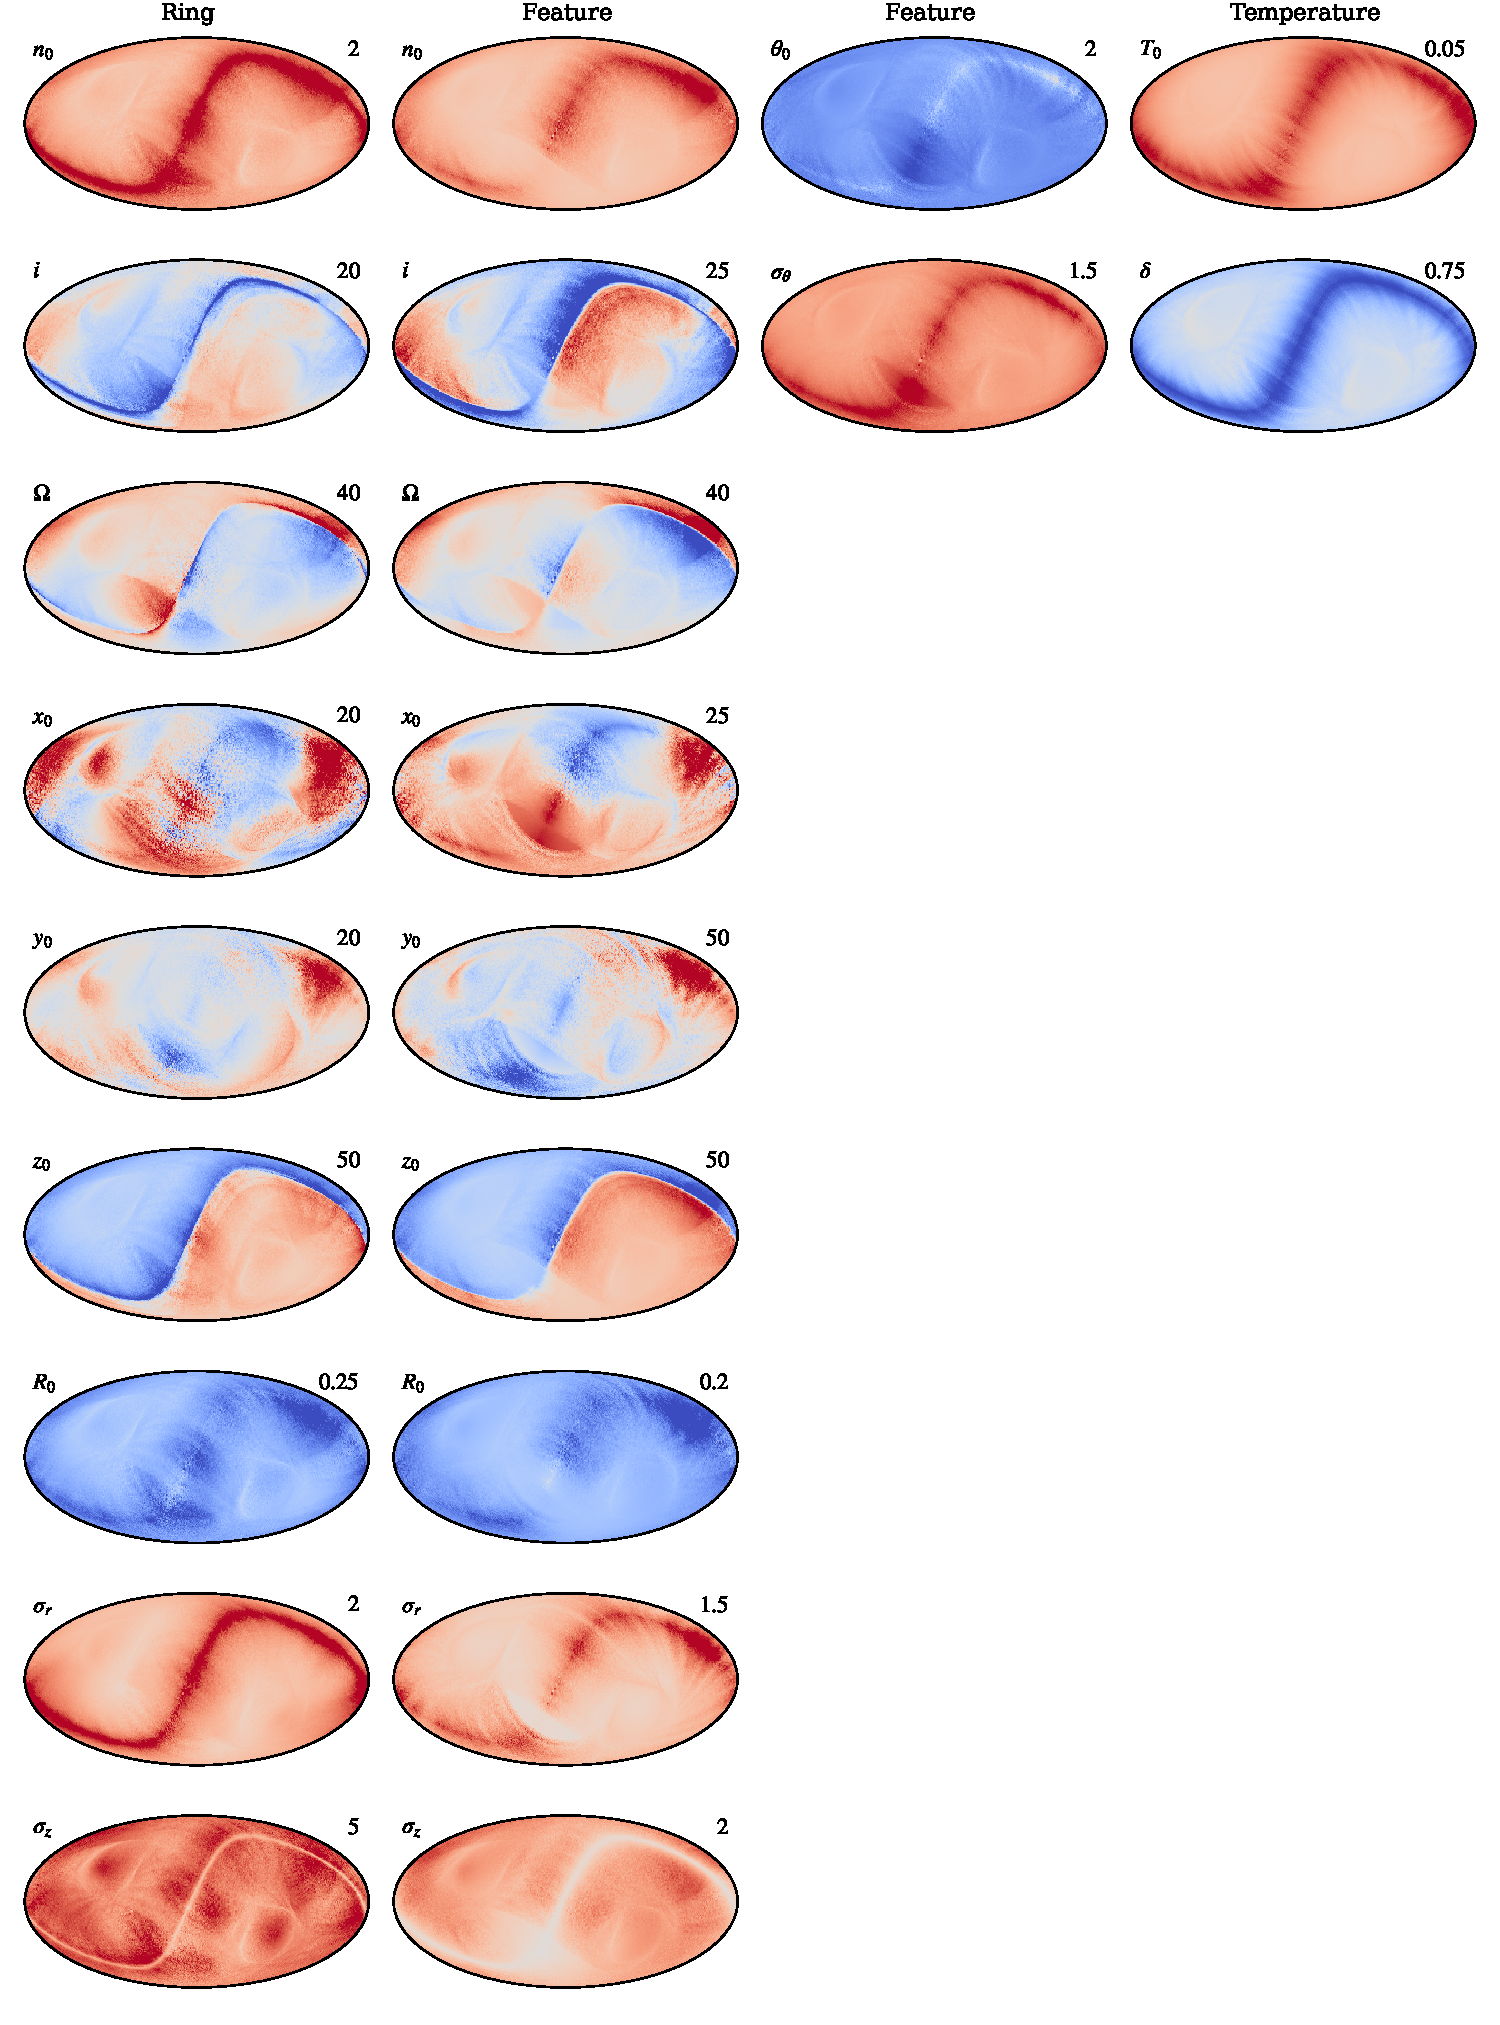
\includegraphics[width=0.84\linewidth]{figs/atlas_2_v2.pdf}
    \caption{ZL parameter atlas showing the effects that changing the circum-solar ring, Earth-trailing feature, and the temperature paramters by $\pm 5\%$ has on the mission-averaged ZL signal. The number associated with each map represents a scaling factor mapping all maps to the same color scale, and inicates how strongly (inversly proportional to the number) the change to a given parameter affects the total ZL signal.}    
    \label{fig:atlas2}
\end{figure*}

\subsection{Goodness-of-fit}
\begin{figure*}
    \centering
    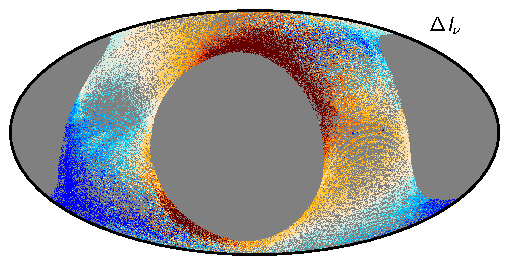
\includegraphics[width=0.49\linewidth]{figs/maptot_06a_week_minus_full.pdf}
    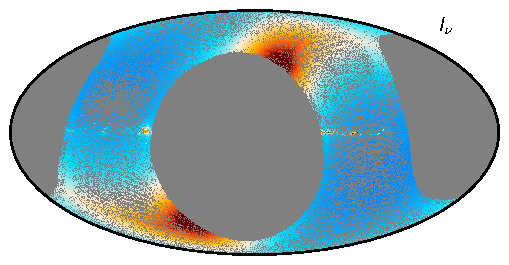
\includegraphics[width=0.49\linewidth]{figs/maptot_06a_week.pdf}\\
    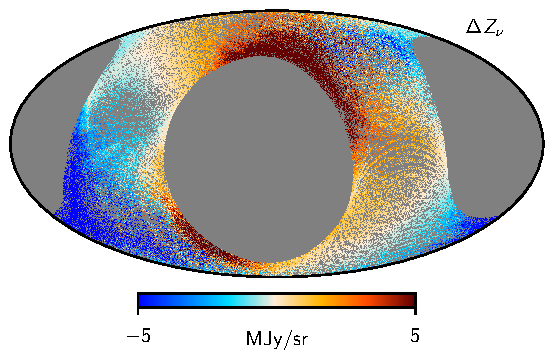
\includegraphics[width=0.49\linewidth]{figs/mapzodi_06a_week_minus_full.pdf}
    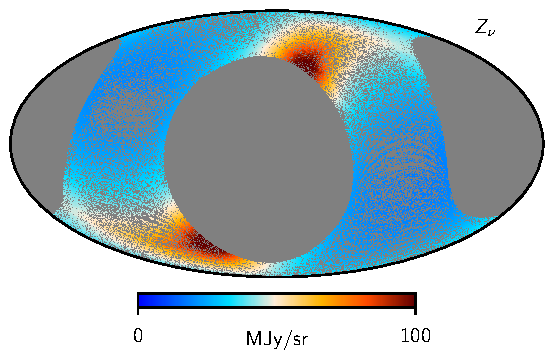
\includegraphics[width=0.49\linewidth]{figs/mapzodi_06a_week.pdf}
    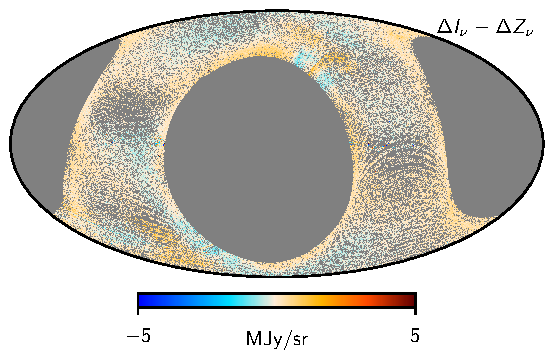
\includegraphics[width=0.49\linewidth]{figs/map_06a_week_minus_full.pdf}
    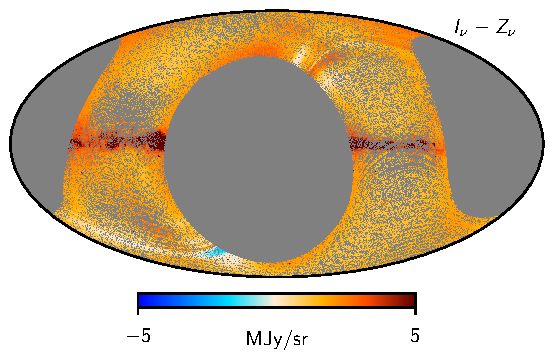
\includegraphics[width=0.49\linewidth]{figs/map_06a_week.pdf}
    \caption{Illustration of the basic sky maps involved in the zodiacal light fitting algorithms adopted by the DIRBE (\emph{left column}) and \Cosmoglobe\ (\emph{right column}) pipelines for one week of $25\,\mu\mathrm{m}$ observations and adopting the K98 model. The DIRBE pipeline used exclusively differences between weekly and full-season maps, both for the observed signal, $\Delta I_{\nu} \equiv I_{\nu}-\left<I_{\nu}\right>$ (\emph{top left}), and the zodiacal light model, $\Delta Z_{\nu} = Z_{\nu}-\left<Z_{\nu}\right>$ (\emph{middle left}), where brackets indicate full-survey averages. Correspondingly, the final $\chi^2$ is defined through $\Delta I_{\nu} - \Delta Z_{\nu}$ (\emph{bottom left}), and is by constrution only sensitive to time-variable signals. 
    In contrast, the basic data element in \Cosmoglobe\ is the full sky signal, $I_{\nu}$ (\emph{top right}), which is fitted with the full zodiacal light model, $Z_{\nu}$ (\emph{middle right}), both modelled in time-domain. The $\chi^2$ the minimizes minimize the total signal-minus-model residual, $I_{\nu}-Z_{\nu}$ (\emph{bottom right}). The main advantage of the DIRBE approach is insensitivity to stationary sky signals, in particular thermal dust and CIB, while the main advantage of the \Cosmoglobe\ approach is a much higher effective signal-to-noise ratio, both to zodiacal light parameters and zero-levels.}
    \label{fig:week_vs_full}
\end{figure*}
\begin{figure}
    \centering
        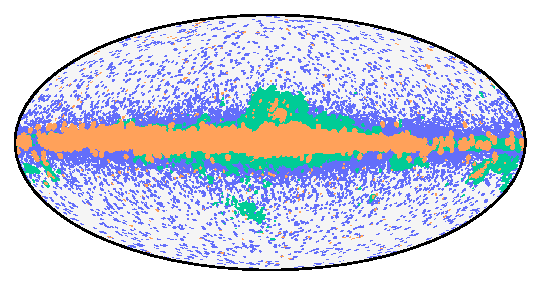
\includegraphics[width=\columnwidth]{figs/mask_zodi_fitting.pdf}
        \caption{Masks applied when fitting zodiacal light parameters for the $2.2\mathrm{\mu m}$, $25\mathrm{\mu m}$ and $240\mathrm{\mu m}$ bands.}
    \label{fig:masks}
\end{figure}
The K98 model was obtained by fitting the model to a set of week-maps. The $\chi^2$ measure used by the DIRBE team is given by
\begin{equation}
    \chi^2_\mathrm{K98} = \Delta I_\nu - \Delta Z_\nu,
\end{equation}
where
\begin{align}
    &\Delta I_\nu = I_\nu - \langle I_\nu \rangle,\\
    &\Delta Z_\nu = Z_\nu - \langle Z_\nu \rangle,
\end{align}
and $I_\nu$ and $Z_\nu$ are the full-mission frequency and ZL estimate maps, and $\Delta I\nu$ and $\Delta Z_\nu$ are the difference between the full-mission and a week frequency and ZL map, respectively. These maps are illustrated in the left column in Figure \ref{fig:week_vs_full}. $\chi^2_\mathrm{K98}$ is by construction only sensitive to time-variable signal, effectively removing the need for a good sky model of the then less well-understood infrared sky. Using week maps instead of the full timestreams has the additional effect of reducing the overall data volume in the fits, which would seem beneficial considering the computing resources available during the early DIRBE analysis. A downside of this method is that the monopole induced by the smooth ZL is removed, resulting in a much weaker signal-to-noise ratio in the ZL parameter estimates and to the zero-levels. In contrast, we fit the data at each time step to the signal minus model residual
\begin{equation}
    \chi^2_\Cosmoglobe\ = I_\nu - Z_\nu.
\end{equation}

To minimize the amount of unmodeled galactic emission that enters our 
ZL parameter estimates, we use strict channel-specific processing masks, masking out the brightest galactic regions. The 1.25, 25, and 240 $\mu$m masks, corresponding to stellar light, ZL, and thermal dust-dominated channels, are shown in Figure \ref{fig:masks}.


\subsection{Minimizing with Powell's method}



\section{Improved zodiacal light model}\label{sect:improved-model}

\begin{figure*}
    \centering
    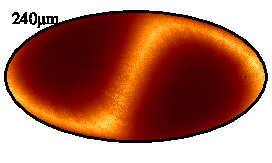
\includegraphics[width=0.22\textwidth]{figs/zodi/zodi_10_tot.pdf}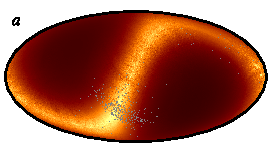
\includegraphics[width=0.22\textwidth]{figs/zodi/zodi_10_a.pdf}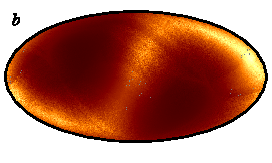
\includegraphics[width=0.22\textwidth]{figs/zodi/zodi_01_b.pdf}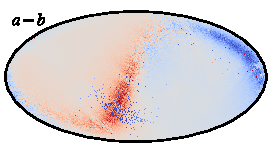
\includegraphics[width=0.22\textwidth]{figs/zodi/zodi_10_a-b.pdf} 
    \vspace{-0.3cm}

    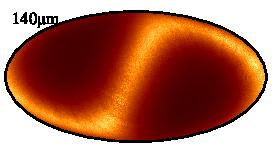
\includegraphics[width=0.22\textwidth]{figs/zodi/zodi_09_tot.pdf}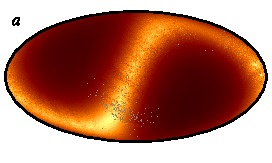
\includegraphics[width=0.22\textwidth]{figs/zodi/zodi_09_a.pdf}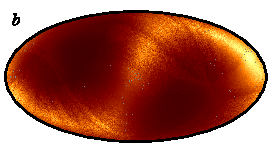
\includegraphics[width=0.22\textwidth]{figs/zodi/zodi_02_b.pdf}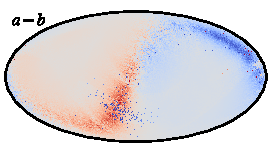
\includegraphics[width=0.22\textwidth]{figs/zodi/zodi_09_a-b.pdf}
    \vspace{-0.3cm}

    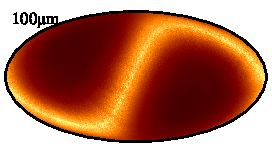
\includegraphics[width=0.22\textwidth]{figs/zodi/zodi_08_tot.pdf}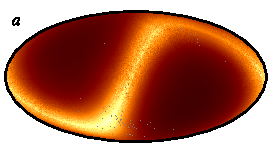
\includegraphics[width=0.22\textwidth]{figs/zodi/zodi_08_a.pdf}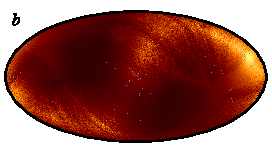
\includegraphics[width=0.22\textwidth]{figs/zodi/zodi_03_b.pdf}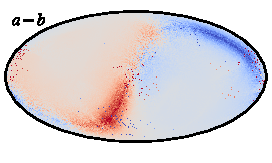
\includegraphics[width=0.22\textwidth]{figs/zodi/zodi_08_a-b.pdf}
    \vspace{-0.3cm}

    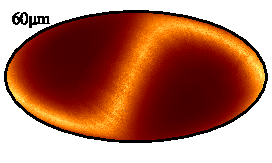
\includegraphics[width=0.22\textwidth]{figs/zodi/zodi_07_tot.pdf}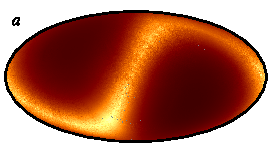
\includegraphics[width=0.22\textwidth]{figs/zodi/zodi_07_a.pdf}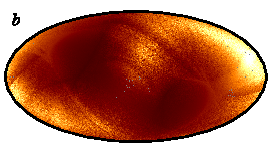
\includegraphics[width=0.22\textwidth]{figs/zodi/zodi_04_b.pdf}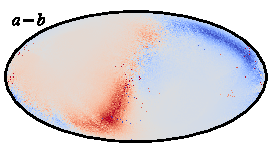
\includegraphics[width=0.22\textwidth]{figs/zodi/zodi_07_a-b.pdf}
    \vspace{-0.3cm}

    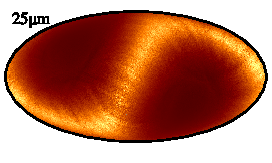
\includegraphics[width=0.22\textwidth]{figs/zodi/zodi_06_tot.pdf}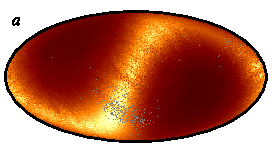
\includegraphics[width=0.22\textwidth]{figs/zodi/zodi_06_a.pdf}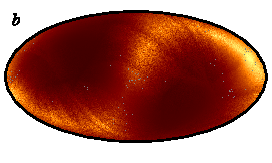
\includegraphics[width=0.22\textwidth]{figs/zodi/zodi_05_b.pdf}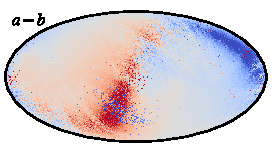
\includegraphics[width=0.22\textwidth]{figs/zodi/zodi_06_a-b.pdf}
    \vspace{-0.3cm}

    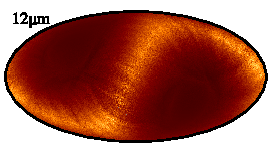
\includegraphics[width=0.22\textwidth]{figs/zodi/zodi_05_tot.pdf}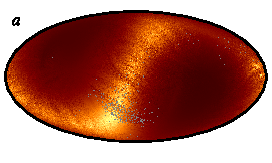
\includegraphics[width=0.22\textwidth]{figs/zodi/zodi_05_a.pdf}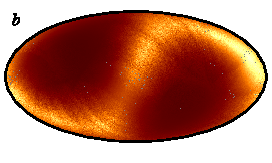
\includegraphics[width=0.22\textwidth]{figs/zodi/zodi_06_b.pdf}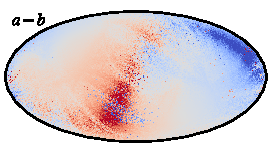
\includegraphics[width=0.22\textwidth]{figs/zodi/zodi_05_a-b.pdf}
    \vspace{-0.3cm}

    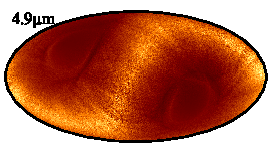
\includegraphics[width=0.22\textwidth]{figs/zodi/zodi_04_tot.pdf}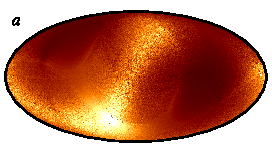
\includegraphics[width=0.22\textwidth]{figs/zodi/zodi_04_a.pdf}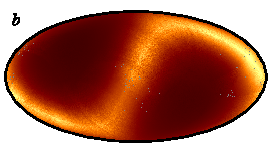
\includegraphics[width=0.22\textwidth]{figs/zodi/zodi_07_b.pdf}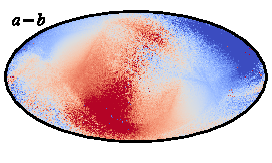
\includegraphics[width=0.22\textwidth]{figs/zodi/zodi_04_a-b.pdf}
    \vspace{-0.3cm}

    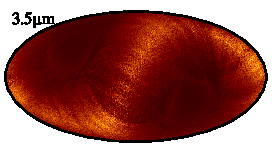
\includegraphics[width=0.22\textwidth]{figs/zodi/zodi_03_tot.pdf}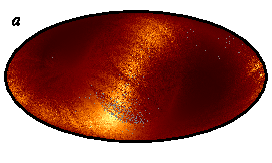
\includegraphics[width=0.22\textwidth]{figs/zodi/zodi_03_a.pdf}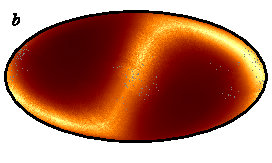
\includegraphics[width=0.22\textwidth]{figs/zodi/zodi_08_b.pdf}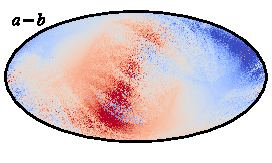
\includegraphics[width=0.22\textwidth]{figs/zodi/zodi_03_a-b.pdf}
    \vspace{-0.3cm}

    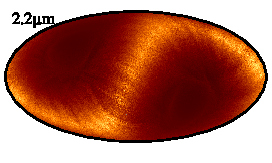
\includegraphics[width=0.22\textwidth]{figs/zodi/zodi_02_tot.pdf}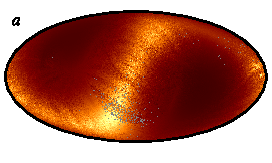
\includegraphics[width=0.22\textwidth]{figs/zodi/zodi_02_a.pdf}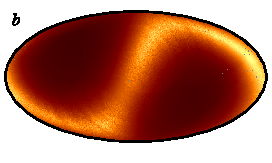
\includegraphics[width=0.22\textwidth]{figs/zodi/zodi_09_b.pdf}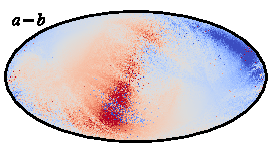
\includegraphics[width=0.22\textwidth]{figs/zodi/zodi_02_a-b.pdf}
    \vspace{-0.3cm}

    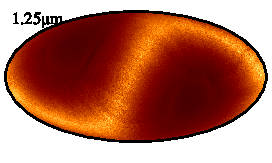
\includegraphics[width=0.22\textwidth]{figs/zodi/zodi_01_tot.pdf}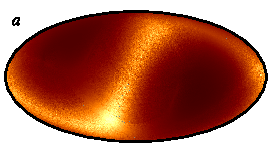
\includegraphics[width=0.22\textwidth]{figs/zodi/zodi_01_a.pdf}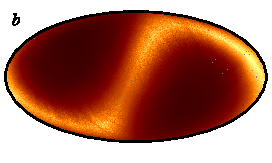
\includegraphics[width=0.22\textwidth]{figs/zodi/zodi_10_b.pdf}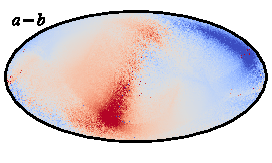
\includegraphics[width=0.22\textwidth]{figs/zodi/zodi_01_a-b.pdf}

    \caption{Zodi frequency maps}
    \label{fig:zodi_freq}
  \end{figure*}

  \begin{figure*}
    \centering
    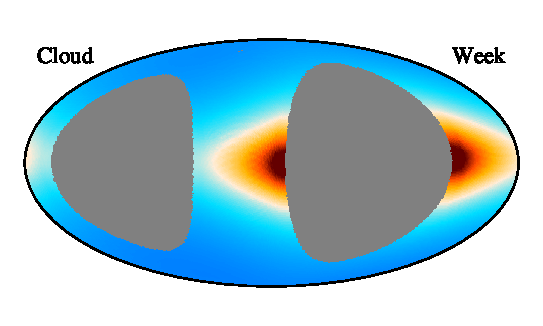
\includegraphics[width=0.88\columnwidth]{figs/zodi_comps/zodi_06_cloud_week.pdf}\includegraphics[width=0.88\columnwidth]{figs/zodi_comps/zodi_06_cloud_full.pdf}

    \vspace{-0.6cm}

    \includegraphics[width=0.88\columnwidth]{figs/zodi_comps/zodi_06_band1_week.pdf}\includegraphics[width=0.88\columnwidth]{figs/zodi_comps/zodi_06_band1_full.pdf}

    \vspace{-0.6cm}

    \includegraphics[width=0.88\columnwidth]{figs/zodi_comps/zodi_06_band2_week.pdf}\includegraphics[width=0.88\columnwidth]{figs/zodi_comps/zodi_06_band2_full.pdf}

    \vspace{-0.6cm}

    \includegraphics[width=0.88\columnwidth]{figs/zodi_comps/zodi_06_band3_week.pdf}\includegraphics[width=0.88\columnwidth]{figs/zodi_comps/zodi_06_band3_full.pdf}

    \vspace{-0.6cm}

    \includegraphics[width=0.88\columnwidth]{figs/zodi_comps/zodi_06_ring_week.pdf}\includegraphics[width=0.88\columnwidth]{figs/zodi_comps/zodi_06_ring_full.pdf}

    \vspace{-0.6cm}

    \includegraphics[width=0.88\columnwidth]{figs/zodi_comps/zodi_06_feature_week.pdf}\includegraphics[width=0.88\columnwidth]{figs/zodi_comps/zodi_06_feature_full.pdf}

    \caption{week map of comps*}
    \label{fig: comp week}
  \end{figure*}

\begin{figure*}
\centering
\includegraphics[width=0.88\columnwidth]{figs/zodi_comps/zodi_sky_98_week.pdf}\includegraphics[width=0.88\columnwidth]{figs/zodi_comps/zodi_cloud_98_week.pdf}
\vspace{-0.6cm}

\includegraphics[width=0.88\columnwidth]{figs/zodi_comps/zodi_zodi_98_week.pdf}\includegraphics[width=0.88\columnwidth]{figs/zodi_comps/zodi_bands_98_week.pdf}
\vspace{-0.6cm}

\includegraphics[width=0.88\columnwidth]{figs/zodi_comps/zodi_res_98_week.pdf}\includegraphics[width=0.88\columnwidth]{figs/zodi_comps/zodi_ring+feature_98_week.pdf}
\caption{week map of comps*}
\label{fig: K98 week comparison}
\end{figure*}

\begin{figure*}
    \centering
    \includegraphics[width=1\textwidth]{figs/total_trace.pdf}
    \caption{Trace plot of all geometrical interplanetary dust paramteres for six independant Markov chains.}
    \label{fig:geo-trace}
\end{figure*}



\begin{table*}
    \centering
    \newcolumntype{C}{ @{}>{${}}r<{{}$}@{} }
    \begin{tabular}{l l *2{rCl}}
    \hline
    \hline
     Parameter & Description & \multicolumn{3}{c}{DIRBE} & \multicolumn{3}{c}{Cosmoglobe DR2} \\ 
     \hline
     \multicolumn{8}{c}{Smooth Cloud}\\
     \hline
     $n_{0, \mathrm{C}}$ [$10^{-7}$ AU$^{-1}$] & Number density & 1.13 &\pm& 0.0064 & 1.13 &\pm& 0.0064\\
     $\alpha$ & Radial power-law exponent \quad& 1.34 &\pm& 0.022 & 1.13 &\pm& 0.0064\\
     $\beta$ & Vertical shape parameter & 4.14 &\pm& 0.067 & 1.13 &\pm& 0.0064\\
     $\gamma$ & Vertical power-law exponent & 0.942 &\pm& 0.025 & 1.13 &\pm& 0.0064\\
     $\mu$ & Widening parameter & 0.189 &\pm& 0.014 & 1.13 &\pm& 0.0064\\
     $i$ [deg] & Inclination & 2.03 &\pm& 0.017 & 1.13 &\pm& 0.0064\\
     $\Omega$ [deg] & Ascending node & 77.7 &\pm& 0.6 & 1.13 &\pm& 0.0064\\
     $X_0$ [$10^{-3}$ AU] & x-offset from the Sun  & 11.9 &\pm& 1.1 & 1.13 &\pm& 0.0064\\
     $Y_0$ [$10^{-3}$ AU] & y-offset from the Sun & 5.48 &\pm& 0.77 & 1.13 &\pm& 0.0064\\
     $Z_0$ [$10^{-3}$ AU] & z-offset from the Sun & -2.15 &\pm& 0.43 & 1.13 &\pm& 0.0064\\
     \hline
     \multicolumn{8}{c}{Dust band 1}\\
     \hline
     $n_{0, \mathrm{B}_1}$ [$10^{-10}$ AU$^{-1}$] & Number density & 5.59 &\pm& 0.72 & 1.13 &\pm& 0.0064\\
     $\delta_{\zeta_{\mathrm{B}_1}}$ [deg] & Shape parameter & 8.78 && Fixed & 1.13 &\pm& 0.0064\\
     $v_{\mathrm{B}_1}$ & Shape parameter & 0.10 && Fixed & 1.13 &\pm& 0.0064\\
     $p_{\mathrm{B}_1}$ & Shape parameter & 4 && Fixed & 0.10 &\pm& 0.0064\\
     $i_{\mathrm{B}_1}$ [deg] & Inclination & 0.56 && Fixed & 0.10 &\pm& 0.0064\\
     $\Omega_{\mathrm{B}_1}$ [deg] & Ascending node & 80 && Fixed & 0.10 &\pm& 0.0064\\
     $\delta_{R_{\mathrm{B}_1}}$ [AU] & Inner radial cutoff & 1.5 && Fixed & 0.10 &\pm& 0.0064\\
     \hline
     \multicolumn{8}{c}{Dust band 2}\\
     \hline
     $n_{0, \mathrm{B}_2}$ [$10^{-9}$ AU$^{-1}$] & Number density & 1.99 &\pm& 0.128 & 1.13 &\pm& 0.0064\\
     $\delta_{\zeta_{\mathrm{B}_2}}$ [deg] & Shape parameter & 1.99 && Fixed & 1.13 &\pm& 0.0064\\
     $v_{\mathrm{B}_2}$ & Shape parameter & 0.9 && Fixed & 1.13 &\pm& 0.0064\\
     $p_{\mathrm{B}_2}$ & Shape parameter & 4 && Fixed & 0.10 &\pm& 0.0064\\
     $i_{\mathrm{B}_2}$ [deg] & Inclination & 1.2 && Fixed & 0.10 &\pm& 0.0064\\
     $\Omega_{\mathrm{B}_2}$ [deg] & Ascending node & 30.3 && Fixed & 0.10 &\pm& 0.0064\\
     $\delta_{R_{\mathrm{B}_2}}$ [AU] & Inner radial cutoff & 0.94 &\pm& 0.025 & 0.10 &\pm& 0.0064\\
     \hline
     \multicolumn{8}{c}{Dust band 3}\\
     \hline
     $n_{0, \mathrm{B}_3}$ [$10^{-10}$ AU$^{-1}$] & Number density & 1.44 &\pm& 0.234 & 1.13 &\pm& 0.0064\\
     $\delta_{\zeta_{\mathrm{B}_3}}$ [deg] & Shape parameter & 15 && Fixed & 1.13 &\pm& 0.0064\\
     $v_{\mathrm{B}_3}$ & Shape parameter & 0.05 && Fixed & 1.13 &\pm& 0.0064\\
     $p_{\mathrm{B}_3}$ & Shape parameter & 4 && Fixed & 0.10 &\pm& 0.0064\\
     $i_{\mathrm{B}_3}$ [deg] & Inclination & 0.8 && Fixed & 0.10 &\pm& 0.0064\\
     $\Omega_{\mathrm{B}_3}$ [deg] & Ascending node & 80 && Fixed & 0.10 &\pm& 0.0064\\
     $\delta_{R_{\mathrm{B}_3}}$ [AU] & Inner radial cutoff & 1.5 && Fixed & 0.10 &\pm& 0.0064\\
     \hline
     \multicolumn{8}{c}{Circum-solar ring}\\
     \hline
     $n_{0, \mathrm{SR}}$ [$10^{-8}$ AU$^{-1}$] & Number density & 1.83 &\pm& 0.127 & 1.13 &\pm& 0.0064\\
     $R_\mathrm{SR}$ [AU] & Radius of peak number density & 1.03 &\pm& 0.00064 & 1.13 &\pm& 0.0064\\
     $\sigma_{r,\mathrm{SR}}$ [AU] & Radial dispersion & 0.025 && Fixed & 1.13 &\pm& 0.0064\\
     $\sigma_{z,\mathrm{SR}}$ [AU] & Vertical dispersion & 0.054 &\pm& 0.0066 & 1.13 &\pm& 0.0064\\
     $i_{\mathrm{SR}}$ [deg] & Inclination & 0.49 &\pm& 0.063 & 0.10 &\pm& 0.0064\\
     $\Omega_{\mathrm{SR}}$ [deg] & Ascending node & 22.3 &\pm& 0.0014 & 0.10 &\pm& 0.0064\\
     \hline
     \multicolumn{8}{c}{Earth-trailing feature}\\
     \hline
     $n_{0, \mathrm{TB}}$ [$10^{-8}$ AU$^{-1}$] & Number density & 1.9 &\pm& 0.142 & 1.13 &\pm& 0.0064\\
     $R_\mathrm{TB}$ [AU] & Radius of peak number density & 1.06 &\pm& 0.011 & 1.13 &\pm& 0.0064\\
     $\sigma_{r,\mathrm{TB}}$ [AU] & Radial dispersion & 0.10 &\pm& 0.0097 & 1.13 &\pm& 0.0064\\
     $\sigma_{z,\mathrm{TB}}$ [AU] & Vertical dispersion & 0.091 &\pm& 0.013 & 1.13 &\pm& 0.0064\\
     $\theta_{\mathrm{TB}}$ [deg] & Longitude with respect to Earth  & -10 && Fixed & 0.10 &\pm& 0.0064\\
     $\sigma_{\theta,\mathrm{TB}}$ [deg] & Longitude dispersion & 12.1 &\pm& 3.4 & 0.10 &\pm& 0.0064\\
     \hline
    \end{tabular}
    \caption{Comparison between best-fit number density and geometrical interplanetary dust parameters in the DIRBE model and our model.}
    \label{table:zodi-params-geo}
    \end{table*}
    
\begin{table*}
    \centering
    \newcolumntype{C}{ @{}>{${}}r<{{}$}@{} }
    \begin{tabular}{l l *2{rCl}}
    \hline
    \hline
     Parameter & Description & \multicolumn{3}{c}{DIRBE} & \multicolumn{3}{c}{Cosmoglobe DR2} \\ 
     \hline
     \multicolumn{8}{c}{Smooth Cloud}\\
     \hline
     $A_1$ & Albedo at 1.25$\mu $m & 0.204 &\pm& 0.0013 & 1.13 &\pm& 0.0064\\
     $A_2$ & Albedo at 2.2$\mu $m & 0.255 &\pm& 0.0017 & 1.13 &\pm& 0.0064\\
     $A_3$ & Albedo at 3.5$\mu $m & 0.210 &\pm& 0.019 & 1.13 &\pm& 0.0064\\
     $A_4$ & Albedo at 4.9$\mu $m  & 0 && Fixed & 1.13 &\pm& 0.0064\\
     $E_3$ & Emissivity at 3.5$\mu $m  & 1.66 &\pm& 0.088 & 1.13 &\pm& 0.0064\\
     $E_4$ & Emissivity at 4.9$\mu $m  & 0.997 &\pm& 0.0036 & 1.13 &\pm& 0.0064\\
     $E_5$ & Emissivity at 12$\mu $m  & 0.958 &\pm& 0.0026 & 1.13 &\pm& 0.0064\\
     $E_6$ & Emissivity at 25$\mu $m  & 1 && Fixed & 1.13 &\pm& 0.0064\\
     $E_7$ & Emissivity at 60$\mu $m  & 0.733 &\pm& 0.0055 & 1.13 &\pm& 0.0064\\
     $E_8$ & Emissivity at 100$\mu $m  & 0.647 &\pm& 0.012 & 1.13 &\pm& 0.0064\\
     $E_9$ & Emissivity at 140$\mu $m  & 0.677 && ? & 1.13 &\pm& 0.0064\\
     $E_10$ & Emissivity at 240$\mu$m    & 0.519 && ? & 1.13 &\pm& 0.0064\\
     \hline
     \multicolumn{8}{c}{Dust bands}\\
     \hline
     \hline
     $A_1$ & Albedo at 1.25$\mu $m & 0.204 && Fixed to smooth cloud & 1.13 &\pm& 0.0064\\
     $A_2$ & Albedo at 2.2$\mu $m & 0.255 && Fixed to smooth cloud & 1.13 &\pm& 0.0064\\
     $A_3$ & Albedo at 3.5$\mu $m & 0.210 && Fixed to smooth cloud & 1.13 &\pm& 0.0064\\
     $A_4$ & Albedo at 4.9$\mu $m  & 0 && Fixed & 1.13 &\pm& 0.0064\\
     $E_3$ & Emissivity at 3.5$\mu $m  & 1.66 && Fixed to smooth cloud & 1.13 &\pm& 0.0064\\
     $E_4$ & Emissivity at 4.9$\mu $m  & 0.359 &\pm& 0.054 & 1.13 &\pm& 0.0064\\
     $E_5$ & Emissivity at 12$\mu $m  & 1.01 &\pm& 0.15 & 1.13 &\pm& 0.0064\\
     $E_6$ & Emissivity at 25$\mu $m  & 1 && Fixed & 1.13 &\pm& 0.0064\\
     $E_7$ & Emissivity at 60$\mu $m  & 1.25 &\pm& 0.3 & 1.13 &\pm& 0.0064\\
     $E_8$ & Emissivity at 100$\mu $m  & 1.52 &\pm& 0.65 & 1.13 &\pm& 0.0064\\
     $E_9$ & Emissivity at 140$\mu $m  & 1.13 && ? & 1.13 &\pm& 0.0064\\
     $E_10$ & Emissivity at 240$\mu $m  & 1.40 && ? & 1.13 &\pm& 0.0064\\
     \hline
     \multicolumn{8}{c}{Circum-solar ring and Earth-trailing feature}\\
     \hline
     \hline
     $A_1$ & Albedo at 1.25$\mu $m & 0.204 && Fixed to smooth cloud & 1.13 &\pm& 0.0064\\
     $A_2$ & Albedo at 2.2$\mu $m & 0.255 && Fixed to smooth cloud & 1.13 &\pm& 0.0064\\
     $A_3$ & Albedo at 3.5$\mu $m & 0.210 && Fixed to smooth cloud & 1.13 &\pm& 0.0064\\
     $A_4$ & Albedo at 4.9$\mu $m  & 0 && Fixed & 1.13 &\pm& 0.0064\\
     $E_3$ & Emissivity at 3.5$\mu $m  & 1.66 && Fixed to smooth cloud & 1.13 &\pm& 0.0064\\
     $E_4$ & Emissivity at 4.9$\mu $m  & 1.06 &\pm& 0.0089 & 1.13 &\pm& 0.0064\\
     $E_5$ & Emissivity at 12$\mu $m  & 1.06 &\pm& 0.00078 & 1.13 &\pm& 0.0064\\
     $E_6$ & Emissivity at 25$\mu $m  & 1 && Fixed & 1.13 &\pm& 0.0064\\
     $E_7$ & Emissivity at 60$\mu $m  & 0.873 &\pm& 0.0042 & 1.13 &\pm& 0.0064\\
     $E_8$ & Emissivity at 100$\mu $m  & 1.1 &\pm& 0.000075 & 1.13 &\pm& 0.0064\\
     $E_9$ & Emissivity at 140$\mu $m  & 1.15 && ? & 1.13 &\pm& 0.0064\\
     $E_10$ & Emissivity at 240$\mu $m  & 0.858 && ? & 1.13 &\pm& 0.0064\\
     \hline
    \end{tabular}
    \caption{Comparison between best-fit spectral parameters in the DIRBE model and our model.}
    \label{table:zodi-params-spectral}
\end{table*}
    

% % INTRODUCTION
% %-------------------------------------------------------------------
% \section{Introduction}
% Zodiacal light (ZL, sometimes zodiacal emission or interplanetary dust emission) is the primary source of diffuse radiation observed in the infrared sky between 1-100 $\mu$m (\cite{leinert1998} and references therein). The light comes from scattering and re-emission of sunlight from interplanetary dust grains. ZL has been the most problematic source of foreground contamination in studies of the Extragalactic Background Light (EBL) the infrared sky due, mainly due to its time-varying nature. Improving our understanding of the interplanetary medium and building better ZL models is arguably the most critical step in making a large part of the infrared sky accessible to cosmological analysis. 

% The current state-of-the-art ZL model is the Kelsall et al. 1998 (K98), which was developed by the DIRBE team for the purpose of removing ZL from their data. It consists of a parametric three-dimensional model of the interplanetary dust distribution with several distinguishable components such as 
% These components were assumed to emit like modified blackbodies and could be evaluated through line-of-sight integrations to simulate the observed zodiacal light. 


% Ever since it was first understood in the 17th century \citep{cassini}, zodiacal light has been a driving force for the exploration of the interplanetary medium. The Diffuse Infrared Background Experiment (DIRBE) instrument, onboard the Cosmic Background Explorer (COBE), found that the zodiacal light could be effectively characterized in the infrared \citep{mather:1994, hauser:1998}. The DIRBE team developed a geometric model that represented the interplanetary medium and its identifiable components.
% These components were assumed to emit like modified blackbodies and could be evaluated through line-of-sight integrations to simulate the observed zodiacal light. This model, detailed in \cite{K98}, (here-after K98), has demonstrated its effectiveness in describing zodiacal light in the infrared and sub-millimeter domains and has been the default modeling used in the cosmology community for the past twenty years. The Planck Collaboration \citep{PLANCK2013, PLANCK2015, PLANCK2018} recently utilized the DIRBE model in their analysis of the High Frequency Instrument (HFI) data. They adapted the model to be applicable at sub-terahertz frequencies by evaluating the K98 model with the HFI scanning strategy and fitting an overall amplitude to model components.

% The ZL is considered a local foreground in CMB studies with the emission originating from the near vicinity of the observer. This is a contrast to more common foregrounds such as the CMB and galactic thermal dust emission, which we assume to be stationary in the sky. Galactic and extragalactic foregrounds can be modeled with a single template describing the structure of the component at some reference frequency. The template can then be scaled to arbitrary frequencies given a description of the component's spectral energy density (SED). Simple models like this does not apply to the zodiacal light, which highly depends on the position and time of observation.
% It is impossible to describe and model the zodiacal light foreground through a single template, applicable to all experiments. Instead, the zodiacal light must be dynamically modeled on a per-experiment basis taking into account the position of the observer within the solar system and the scanning strategy. 

% The main highlight of this work is that we are able to produce a better zodiacal light model with much smaller residuals in the frequency maps using only the same zodiacal light-contaminated data used by the DIRBE team in their original analysis. We attribute most of this success to the Cosmoglobe effort of joint global Bayesian analysis of the time-ordered DIRBE data along with maps and point source catalogs from HFI, FIRAS, and WISE. This results in a much better constrained sky model than what was possible at the time of the original DIRBE analysis, making it easier to distinguish the zodiacal light from other signal sources. Additionally, when fitting the zodiacal light model parameters, the DIRBE team used week maps differenced by the full survey sky map. While this removes all static signals from the sky, it also kills much of the effective signal-to-noise ratio for both zodiacal light parameters and the zero levels. In the Cosmoglobe approach, we fit all zodiacal light parameters directly to the timestreams, making it easier to resolve the degeneracies of the geometric interplanetary dust parameters. 

% This goes to show that even when only using archival data, it is possible to create more robust descriptions of the interplanetary medium and the observed zodiacal light. In coming Cosmoglobe data releases we will include more zodiacal light-contaminated time-ordered data from experiments such as AKARI and IRAS, which will help break many of the geometric parameter degeneracies in the interplanetary dust model due to the complimentary scanning strategies of the respective experiments.

% In this paper, we will detail the zodiacal light modeling approach used in the Commander framework during the production of Cosmoglobe DR2. Furthermore, the perhaps greatest result from this works comes from the fitting of the model parameters from a Bayesian perspective, utilizing all DIRBE bands jointly along with HFI, FIRAS and WISE data to produce the best zodiacal light model of the infrared sky. 
% In Sect. 2 we describe zodiacal light model in terms of the interplanetary dust models, source functions, and line-of-sight integrations. 
% Additionally, introduce and interpret the zodiacal light in the DIRBE time-ordered data. Finally we discuss the sampling techniques used to fit the many zodiacal light model parameters from a Bayesian perspective. In Sect. 3 we reanalyze the DIRBE data using the K98 model as derived by the DIRBE team, and see that we recover their results. 
% In Sect. 4 we explore extensions to the K98 model by lifting some of the constraints set on the model parameter by the DIRBE team, and including some of the more physical descriptions of the zodiacal components from \cite{RRM}. These extended models are referred to as model A and B, where model A is the relaxed K98 model, while model B is a more complex model with additional modifications.



% \subsection{Rowan-Robinson and May (RRM) model}
% In the RRM model, the components are described in terms of the radial distance from the component center $r_c$ and the the latitude above the symmetry-plane $\beta_0$. The transformation between the two angular and cartesian representations are given by $z_c = r_c \sin{\beta_0}$, 
% \begin{equation}
%     \beta_0 = \arctan\left(\frac{z_c}{r_c}\right).
% \end{equation}

% \subsubsection{The fan}
% The fan is the RRM equivalent of the diffuse cloud in the K98 model. The density of the fan is described in a separable form similar to the diffuse cloud
% \begin{equation}
%     n_{\mathrm{Fan}}\left(r_\mathrm{Fan}, \beta_0\right)=n_0 r_\mathrm{Fan}^{-\gamma} f\left(\beta_0\right),
% \end{equation}
% but the vertical distribution is rather given as 
% \begin{equation}
% f\left(\beta_0\right)=\left(\cos \beta_0\right)^Q \exp \left(-P \sin \left|\beta_0\right|^{\xi}\right),
% \end{equation}
% where
% \begin{equation}\ 
% \xi= \begin{cases}
%     2 - |z_{\mathrm{Fan}}/z_{\mathrm{Fan}, 0}| \mid & \text { for }|z_\mathrm{Fan}|<z_{\mathrm{Fan}, 0} \\     1 & \text { otherwise },
% \end{cases}
% \end{equation}
% Add more components if we use them.
    
% \begin{figure}
%     \centering
%          \includegraphics[width=\linewidth]{figs/zodi_obs_diff.pdf}
%         \caption{Difference in simulated zodiacal light between an observed at the center of Earth and an observer moved 900km in the positive z-direction from the center of Earth.}
%     \label{fig: z}
% \end{figure}

% \begin{figure}
%     \centering
%         \includegraphics[width=\columnwidth]{figs/mask_zodi_fitting.pdf}
%         \caption{Masks applied when fitting zodiacal light parameters for the $2.2\mathrm{\mu m}$, $25\mathrm{\mu m}$ and $240\mathrm{\mu m}$ bands.}
%     \label{fig:masks}
% \end{figure}

% \begin{figure*}
%     \centering
%     \includegraphics[width=0.22\textwidth]{figs/zodi/zodi_10_tot.pdf}\includegraphics[width=0.22\textwidth]{figs/zodi/zodi_10_a.pdf}\includegraphics[width=0.22\textwidth]{figs/zodi/zodi_01_b.pdf}\includegraphics[width=0.22\textwidth]{figs/zodi/zodi_10_a-b.pdf} 
%     \vspace{-0.3cm}

%     \includegraphics[width=0.22\textwidth]{figs/zodi/zodi_09_tot.pdf}\includegraphics[width=0.22\textwidth]{figs/zodi/zodi_09_a.pdf}\includegraphics[width=0.22\textwidth]{figs/zodi/zodi_02_b.pdf}\includegraphics[width=0.22\textwidth]{figs/zodi/zodi_09_a-b.pdf}
%     \vspace{-0.3cm}

%     \includegraphics[width=0.22\textwidth]{figs/zodi/zodi_08_tot.pdf}\includegraphics[width=0.22\textwidth]{figs/zodi/zodi_08_a.pdf}\includegraphics[width=0.22\textwidth]{figs/zodi/zodi_03_b.pdf}\includegraphics[width=0.22\textwidth]{figs/zodi/zodi_08_a-b.pdf}
%     \vspace{-0.3cm}

%     \includegraphics[width=0.22\textwidth]{figs/zodi/zodi_07_tot.pdf}\includegraphics[width=0.22\textwidth]{figs/zodi/zodi_07_a.pdf}\includegraphics[width=0.22\textwidth]{figs/zodi/zodi_04_b.pdf}\includegraphics[width=0.22\textwidth]{figs/zodi/zodi_07_a-b.pdf}
%     \vspace{-0.3cm}

%     \includegraphics[width=0.22\textwidth]{figs/zodi/zodi_06_tot.pdf}\includegraphics[width=0.22\textwidth]{figs/zodi/zodi_06_a.pdf}\includegraphics[width=0.22\textwidth]{figs/zodi/zodi_05_b.pdf}\includegraphics[width=0.22\textwidth]{figs/zodi/zodi_06_a-b.pdf}
%     \vspace{-0.3cm}

%     \includegraphics[width=0.22\textwidth]{figs/zodi/zodi_05_tot.pdf}\includegraphics[width=0.22\textwidth]{figs/zodi/zodi_05_a.pdf}\includegraphics[width=0.22\textwidth]{figs/zodi/zodi_06_b.pdf}\includegraphics[width=0.22\textwidth]{figs/zodi/zodi_05_a-b.pdf}
%     \vspace{-0.3cm}

%     \includegraphics[width=0.22\textwidth]{figs/zodi/zodi_04_tot.pdf}\includegraphics[width=0.22\textwidth]{figs/zodi/zodi_04_a.pdf}\includegraphics[width=0.22\textwidth]{figs/zodi/zodi_07_b.pdf}\includegraphics[width=0.22\textwidth]{figs/zodi/zodi_04_a-b.pdf}
%     \vspace{-0.3cm}

%     \includegraphics[width=0.22\textwidth]{figs/zodi/zodi_03_tot.pdf}\includegraphics[width=0.22\textwidth]{figs/zodi/zodi_03_a.pdf}\includegraphics[width=0.22\textwidth]{figs/zodi/zodi_08_b.pdf}\includegraphics[width=0.22\textwidth]{figs/zodi/zodi_03_a-b.pdf}
%     \vspace{-0.3cm}

%     \includegraphics[width=0.22\textwidth]{figs/zodi/zodi_02_tot.pdf}\includegraphics[width=0.22\textwidth]{figs/zodi/zodi_02_a.pdf}\includegraphics[width=0.22\textwidth]{figs/zodi/zodi_09_b.pdf}\includegraphics[width=0.22\textwidth]{figs/zodi/zodi_02_a-b.pdf}
%     \vspace{-0.3cm}

%     \includegraphics[width=0.22\textwidth]{figs/zodi/zodi_01_tot.pdf}\includegraphics[width=0.22\textwidth]{figs/zodi/zodi_01_a.pdf}\includegraphics[width=0.22\textwidth]{figs/zodi/zodi_10_b.pdf}\includegraphics[width=0.22\textwidth]{figs/zodi/zodi_01_a-b.pdf}

%     \caption{Zodi frequency maps}
%     \label{fig:zodi_freq}
%   \end{figure*}

%   \begin{figure*}
%     \centering
%     \includegraphics[width=0.9\columnwidth]{figs/zodi_comps/zodi_06_cloud_week.pdf}\includegraphics[width=0.9\columnwidth]{figs/zodi_comps/zodi_06_cloud_full.pdf}

%     \vspace{-0.6cm}

%     \includegraphics[width=0.9\columnwidth]{figs/zodi_comps/zodi_06_band1_week.pdf}\includegraphics[width=0.9\columnwidth]{figs/zodi_comps/zodi_06_band1_full.pdf}

%     \vspace{-0.6cm}

%     \includegraphics[width=0.9\columnwidth]{figs/zodi_comps/zodi_06_band2_week.pdf}\includegraphics[width=0.9\columnwidth]{figs/zodi_comps/zodi_06_band2_full.pdf}

%     \vspace{-0.6cm}

%     \includegraphics[width=0.9\columnwidth]{figs/zodi_comps/zodi_06_band3_week.pdf}\includegraphics[width=0.9\columnwidth]{figs/zodi_comps/zodi_06_band3_full.pdf}

%     \vspace{-0.6cm}

%     \includegraphics[width=0.9\columnwidth]{figs/zodi_comps/zodi_06_ring_week.pdf}\includegraphics[width=0.9\columnwidth]{figs/zodi_comps/zodi_06_ring_full.pdf}

%     \vspace{-0.6cm}

%     \includegraphics[width=0.9\columnwidth]{figs/zodi_comps/zodi_06_feature_week.pdf}\includegraphics[width=0.9\columnwidth]{figs/zodi_comps/zodi_06_feature_full.pdf}

%     \caption{week map of comps*}
%     \label{fig: comp week}
%   \end{figure*}

% \begin{figure*}
% \centering
% \includegraphics[width=0.9\columnwidth]{figs/zodi_comps/zodi_sky_98_week.pdf}\includegraphics[width=0.9\columnwidth]{figs/zodi_comps/zodi_cloud_98_week.pdf}
% \vspace{-0.6cm}

% \includegraphics[width=0.9\columnwidth]{figs/zodi_comps/zodi_zodi_98_week.pdf}\includegraphics[width=0.9\columnwidth]{figs/zodi_comps/zodi_bands_98_week.pdf}
% \vspace{-0.6cm}

% \includegraphics[width=0.9\columnwidth]{figs/zodi_comps/zodi_res_98_week.pdf}\includegraphics[width=0.9\columnwidth]{figs/zodi_comps/zodi_ring+feature_98_week.pdf}
% \caption{week map of comps*}
% \label{fig: K98 week comparison}
% \end{figure*}



% \subsection{DIRBE data}
% Discuss data used for sampling of the model. Talk about time-order processing, downsampling, thinning, etc.

% %\subsection{Difficulties with sampling and degeneracies in the interplanetary dust model parameters}
% See atlases in figure \ref{fig: atlas1} and \ref{fig: atlas2} for degeneracies in the interplanetary dust model parameters.

% \subsection{Sampling techniques}

% \begin{figure*}
%     \centering
%     \includegraphics{figs/zodi_params_new.pdf}
%     \caption{A subset of the estimated zodiacal light parameters fit in this work.}
%     \label{fig: zodi_trace}

% \end{figure*}



% The approach we will use Gibbs sample each of the model parameters. This means that we propose a change to one model parameter, estimate the zodiacal emission over the full timestream of each ten DIRBE bands, compute a chi-squared and accept/reject. We perform N such proposals before we move on the the next parameter. Since the zodiacal emission is mostly very smooth on the sky, we can afford to downsample the TOD timestream before evaluating the zodiacal emission. For the diffuse cloud and the dust bands we downsample the TODS by X. For the circum-solar ring and the Earth-trailing feature, which are less smooth, and harder to constrain, we downsample the TODS by X. The downsampled TODS are subtracted by the \Cosmoglobe\ skymodel, and recomputed after after each parameter evaluation. 








% \section{Reanalysis of the K98 zodiacal light model}



% \begin{figure*}
% 	\centering
% 	\includegraphics[width=0.8\linewidth]{figs/zodi_diff.pdf}
% 	\caption{Half-mission model. Columns 1 and 2 are the prediction of the zodiacal emission for each band for the first and second half of the DIRBE mission. Column 3 is the difference between these two columns, and column 4 is the difference between the two zodi-subtracted half-mission maps}
% 	\label{fig: zodi_HM}
% \end{figure*}

% \begin{figure*}
%     \centering
% 	 \includegraphics[width=0.8\linewidth]{figs/tod_zodi_residuals.pdf}
% 	\caption{Data-minus-model residual for \cosmoglobe\ results (CG, black) and the official \cite{K98} model (K98, orange), as a function of ecliptic latitude, Galactic latitude, and Solar elongation. The offset for \cosmoglobe\ and the K98 model are listed on the left and right axes of each row, respectively. The \cosmoglobe\ and K98 values are horizontally offset left and right respectively for clarity.}
%       \label{fig: zodi_timestream}
%   \end{figure*}

% \begin{table*}
%     % \renewcommand{\arraystretch}{1.1} % Default value: 1
%     \begin{center}
%     \small
%     \caption{Best fit geometrical interplanetary dust parameters as fit by K98 and us.}
%     \label{table:zodi parameters}
%     \begin{tabular}{
%         l 
%         l 
%         >{\collectcell{}}r<{\endcollectcell}
%         @{${}\pm{}$}
%         >{\collectcell{}}l<{\endcollectcell}
%         >{\collectcell{}}r<{\endcollectcell}
%         @{${}\pm{}$}
%         >{\collectcell{}}l<{\endcollectcell}
%         >{\collectcell{}}r<{\endcollectcell}
%         @{${}\pm{}$}
%         >{\collectcell{}}l<{\endcollectcell}
%     }
%     \hline \hline
%     Parameter & Description & \multicolumn{2}{c}{K98} & \multicolumn{2}{c}{Model A} & \multicolumn{2}{c}{Model B} \\
%     \hline
%     \multicolumn{8}{c}{All zodiacal components}\\
%     \hline
%     $T_0$ [K]     & Temperature at 1 AU    & \multicolumn{2}{c}{286} & \multicolumn{2}{c}{286} & \multicolumn{2}{c}{286}\\
%     $\delta$      & Temperature power-law exponent    & \multicolumn{2}{c}{0.467} & \multicolumn{2}{c}{0.467} & \multicolumn{2}{c}{0.467}\\
%     \hline
%     \multicolumn{8}{c}{Diffuse cloud}\\
%     \hline
%     $n_0$ [$10^{-7}$ AU$^{-1}$]     & Density at 1 AU               & 1.13 & 0.0064           & 1.13 & 0.0064         & 1.13 & 0.0064\\
%     $\alpha$                        & Radial power-law exponent     & 1.34 & 0.022            & 1.34 & 0.022          & 1.34 & 0.022\\
%     $\beta$                         & Vertical shape parameter      & 4.14 & 0.067            & 4.14 & 0.067          & 4.14 & 0.067\\
%     $\gamma$                        & Vertical power-law exponent   & 0.942 & 0.025           & 0.942 & 0.025         & 0.942 & 0.025\\
%     $\mu$                           & Widening parameter            & 0.189 & 0.014           & 0.189 & 0.014         & 0.189 & 0.014\\
%     $i$ [deg]                       & Inclination                   & 2.03 & 0.017            & 2.03 & 0.017          & 2.03 & 0.017\\
%     $\Omega$ [deg]                  & Ascending node                & 77.7 & 0.6              & 77.7 & 0.6            & 77.7 & 0.6\\
%     $X_0$ [$10^{-3}$ AU]            & x offset from Sun             & 11.9 & 1.1 & 11.9 & 11.9 & 1.1 & 11.9 \\ 
%     $Y_0$ [$10^{-3}$ AU]            & y offset from Sun             & 5.48 & 0.77 & 5.48 & 5.48 & 0.77 & 5.48 \\ 
%     $Z_0$ [$10^{-3}$ AU]            & z offset from Sun             & 2.15 & 0.43 & 2.15 & 2.15 & 0.43 & 2.15 \\ 
%     \hline
%     \multicolumn{8}{c}{Asteroidal dust band 1}\\
%     \hline
%     $n_0$ [$10^{-10}$ AU$^{-1}$]  & Density at 3 AU               & 5.59 & 0.72                 & 5.59 & 0.72               & 5.59 & 0.72\\
%     $\delta_{\zeta_{B}}$ [deg]    & Shape parameter               & \multicolumn{2}{c}{8.78}    & \multicolumn{2}{c}{8.78}  & \multicolumn{2}{c}{8.78}\\
%     $v_{B}$                       & Shape parameter               & \multicolumn{2}{c}{0.1}     & \multicolumn{2}{c}{0.1}   & \multicolumn{2}{c}{0.1}\\
%     $p_{B}$                       & Shape parameter               & \multicolumn{2}{c}{4}       & \multicolumn{2}{c}{4}     & \multicolumn{2}{c}{4}\\
%     $i_{B}$ [deg]                 & Inclination                   & \multicolumn{2}{c}{0.56}    & \multicolumn{2}{c}{0.56}  & \multicolumn{2}{c}{0.56}\\
%     $\Omega_{B}$ [deg]            & Ascending node                & \multicolumn{2}{c}{80}      & \multicolumn{2}{c}{80}    & \multicolumn{2}{c}{80}\\
%     $\delta_{R_{B}}$ [AU]         & Inner radial cutoff           & \multicolumn{2}{c}{1.5}     & \multicolumn{2}{c}{1.5}   & \multicolumn{2}{c}{1.5}\\
%     \hline
%     \multicolumn{8}{c}{Asteroidal dust band 2}\\
%     \hline
%     $n_0$ [$10^{-9}$ AU$^{-1}$]   & Density at 3 AU               & 1.99 & 0.128                & 1.99 & 0.128              & 1.99 & 0.128\\
%     $\delta_{\zeta_{B}}$ [deg]    & Shape parameter               & \multicolumn{2}{c}{8.78}    & \multicolumn{2}{c}{8.78}  & \multicolumn{2}{c}{8.78}\\
%     $v_{B}$                       & Shape parameter               & \multicolumn{2}{c}{0.9}     & \multicolumn{2}{c}{0.9}   & \multicolumn{2}{c}{0.9}\\
%     $p_{B}$                       & Shape parameter               & \multicolumn{2}{c}{4}       & \multicolumn{2}{c}{4}     & \multicolumn{2}{c}{4}\\
%     $i_{B}$ [deg]                 & Inclination                   & \multicolumn{2}{c}{1.2}     & \multicolumn{2}{c}{1.2}   & \multicolumn{2}{c}{1.2}\\
%     $\Omega_{B}$ [deg]            & Ascending node                & \multicolumn{2}{c}{30.3}    & \multicolumn{2}{c}{30.3}  & \multicolumn{2}{c}{30.3}\\
%     $\delta_{R_{B}}$ [AU]         & Inner radial cutoff           & \multicolumn{2}{c}{0.94}    & \multicolumn{2}{c}{0.94}  & \multicolumn{2}{c}{0.94}\\
%     \hline
%     \multicolumn{8}{c}{Asteroidal dust band 3}\\
%     \hline
%     $n_0$ [$10^{-10}$ AU$^{-1}$]  & Density at 3 AU               & 1.44 & 0.234                & 1.44 & 0.234              & 1.44 & 0.234  \\
%     $\delta_{\zeta_{B}}$ [deg]    & Shape parameter               & \multicolumn{2}{c}{15}      & \multicolumn{2}{c}{15}    & \multicolumn{2}{c}{15}\\
%     $v_{B}$                       & Shape parameter               & \multicolumn{2}{c}{0.05}    & \multicolumn{2}{c}{0.05}  & \multicolumn{2}{c}{0.05}\\
%     $p_{B}$                       & Shape parameter               & \multicolumn{2}{c}{4}       & \multicolumn{2}{c}{4}     & \multicolumn{2}{c}{4}\\
%     $i_{B}$ [deg]                 & Inclination                   & \multicolumn{2}{c}{0.8}     & \multicolumn{2}{c}{0.8}   & \multicolumn{2}{c}{0.8}\\
%     $\Omega_{B}$ [deg]            & Ascending node                & \multicolumn{2}{c}{80}      & \multicolumn{2}{c}{80}    & \multicolumn{2}{c}{80}\\
%     $\delta_{R_{B}}$ [AU]         & Inner radial cutoff           & \multicolumn{2}{c}{1.5}     & \multicolumn{2}{c}{1.5}   & \multicolumn{2}{c}{1.5}\\
%     \hline
%     \multicolumn{8}{c}{Circumsolar Ring}\\
%     \hline
%     $n_\mathrm{SR}$ [$10^{-8}$ AU$^{-1}$]   & Density at 1 AU           & 1.83 & 0.127              & 1.83 & 0.127              & 1.83 & 0.127\\
%     $R_\mathrm{SR}$ [AU]                    & Radius of peak density    & 1.03 & 0.00016            & 1.03 & 0.00016            & 1.03 & 0.00016\\
%     $\sigma_\mathrm{rSR}$ [AU]              & Radial dispersion         & \multicolumn{2}{c}{0.025} & \multicolumn{2}{c}{0.025} & \multicolumn{2}{c}{0.025}\\
%     $\sigma_\mathrm{zSR}$ [AU]              & Vertical dispersion       & 0.054 & 0.0066            & 0.054 & 0.0066            & 0.054 & 0.0066\\
%     $i_\mathrm{RB}$ [deg]                   & Inclination               & 0.49  & 0.063             & 0.49  & 0.063             & 0.49  & 0.063\\
%     $\Omega_\mathrm{RB}$ [deg]              & Ascending node            & 22.3  & 0.0014            & 22.3 & 0.0014             & 22.3 & 0.0014\\
%     \hline
%     \multicolumn{8}{c}{Trailing Feature}\\
%     \hline
%     $n_\mathrm{TB}$ [$10^{-8}$ AU$^{-1}$]   & Density at 1 AU                   & 1.9 & 0.142 & 1.9 & 0.142 & 1.9 & 0.142\\
%     $R_\mathrm{TB}$ [AU]                    & Radius of peak density            & 1.06 & 0.011 & 1.06 & 0.011 & 1.06 & 0.011\\
%     $\sigma_\mathrm{rTB}$ [AU]              & Radial dispersion                 &  0.10 & 0.0097 & 0.10 & 0.0097 & 0.10 & 0.0097\\
%     $\sigma_\mathrm{zTB}$ [AU]              & Vertical dispersion               & 0.091 &  0.013 & 0.091 &  0.013 & 0.091 &  0.013\\
%     $\theta_\mathrm{TB}$ [deg]              & Longitude with respect to Earth   & \multicolumn{2}{c}{-10} & \multicolumn{2}{c}{-10} & \multicolumn{2}{c}{-10}\\
%     $\sigma_\mathrm{\theta TB}$ [deg]       & Longitude dispersion              & 12.1 & 3.4 & 12.1 & 3.4 & 12.1 & 3.4\\
%     \hline    
%     \end{tabular}
%     \end{center}
% \end{table*}


% \begin{table*}
%     % \renewcommand{\arraystretch}{1.1} % Default value: 1
%     \begin{center}
%     \small
%     \caption{Best fit zodiacal light source parameters from this analysis and the K98 model.}
%     \label{table:zodi parameters}
%     \begin{tabular}{
%         l 
%         >{\collectcell\Num}r<{\endcollectcell}
%         @{${}\pm{}$}
%         >{\collectcell\Num}l<{\endcollectcell}
%         >{\collectcell\Num}r<{\endcollectcell}
%         @{${}\pm{}$}
%         >{\collectcell\Num}l<{\endcollectcell}
%         >{\collectcell\Num}r<{\endcollectcell}
%         @{${}\pm{}$}
%         >{\collectcell\Num}l<{\endcollectcell}
%         >{\collectcell\Num}r<{\endcollectcell}
%         @{${}\pm{}$}
%         >{\collectcell\Num}l<{\endcollectcell}
%         >{\collectcell\Num}r<{\endcollectcell}
%         @{${}\pm{}$}
%         >{\collectcell\Num}l<{\endcollectcell}
%         >{\collectcell\Num}r<{\endcollectcell}
%         @{${}\pm{}$}
%         >{\collectcell\Num}l<{\endcollectcell}
%     }
%     \hline \hline
%     Channel [$\mu$m] & \multicolumn{2}{c}{Diffuse Cloud} & \multicolumn{2}{c}{Dust band 1} & \multicolumn{2}{c}{Dust band 2} & \multicolumn{2}{c}{Dust band 3} & \multicolumn{2}{c}{Circumsolar ring} & \multicolumn{2}{c}{Trailing feature} \\
%     \hline
%     \multicolumn{13}{c}{Emissivity}\\
%     \hline
%     3.5  & 1.66 & 0.088 & \multicolumn{2}{c}{1} & \multicolumn{2}{c}{1} & \multicolumn{2}{c}{1} & \multicolumn{2}{c}{1} & \multicolumn{2}{c}{1} \\
%     4.9  & 0.997 & 0.0036 & \multicolumn{2}{c}{1} & \multicolumn{2}{c}{1} & \multicolumn{2}{c}{1} & \multicolumn{2}{c}{1} & \multicolumn{2}{c}{1} \\
%     12  & 0.958 & 0.002 & \multicolumn{2}{c}{1} & \multicolumn{2}{c}{1} & \multicolumn{2}{c}{1} & \multicolumn{2}{c}{1} & \multicolumn{2}{c}{1} \\
%     25  & \multicolumn{2}{c}{1} & \multicolumn{2}{c}{1} & \multicolumn{2}{c}{1} & \multicolumn{2}{c}{1} & \multicolumn{2}{c}{1} & \multicolumn{2}{c}{1} \\
%     60  & 0.733 & 0.0055 & \multicolumn{2}{c}{1} & \multicolumn{2}{c}{1} & \multicolumn{2}{c}{1} & \multicolumn{2}{c}{1} & \multicolumn{2}{c}{1} \\
%     100  & 0.647 & 0.012 & \multicolumn{2}{c}{1} & \multicolumn{2}{c}{1} & \multicolumn{2}{c}{1} & \multicolumn{2}{c}{1} & \multicolumn{2}{c}{1} \\
%     140  & \multicolumn{2}{c}{1} & \multicolumn{2}{c}{1} & \multicolumn{2}{c}{1} & \multicolumn{2}{c}{1} & \multicolumn{2}{c}{1} & \multicolumn{2}{c}{1} \\
%     240  & \multicolumn{2}{c}{1} & \multicolumn{2}{c}{1} & \multicolumn{2}{c}{1} & \multicolumn{2}{c}{1} & \multicolumn{2}{c}{1} & \multicolumn{2}{c}{1} \\
%     \hline
%     \multicolumn{13}{c}{Albedo}\\
%     \hline
%     1.25  & \multicolumn{2}{c}{1} & \multicolumn{2}{c}{1} & \multicolumn{2}{c}{1} & \multicolumn{2}{c}{1} & \multicolumn{2}{c}{1} & \multicolumn{2}{c}{1} \\
%     2.2  & \multicolumn{2}{c}{1} & \multicolumn{2}{c}{1} & \multicolumn{2}{c}{1} & \multicolumn{2}{c}{1} & \multicolumn{2}{c}{1} & \multicolumn{2}{c}{1} \\
%     3.5  & \multicolumn{2}{c}{1} & \multicolumn{2}{c}{1} & \multicolumn{2}{c}{1} & \multicolumn{2}{c}{1} & \multicolumn{2}{c}{1} & \multicolumn{2}{c}{1} \\
%     \end{tabular}
%     \end{center}
% \end{table*}


% \clearpage
% \section{Extended zodiacal light models}

% \subsection{Generalized K98 modelling}

% \subsection{RRM modelling}

% %\subsection{Interplanetary dust model}
% Describe the model components used and tabulate all parameters fit.

% %\subsection{Spectral parameters (emissivities / albedos)}

% %\subsection{Zodi subtracted DIRBE maps and timestreams}

\section{Conclusions}


\begin{acknowledgements}
 The current work has received funding from the European
  Union’s Horizon 2020 research and innovation programme under grant
  agreement numbers 819478 (ERC; \textsc{Cosmoglobe}) and 772253 (ERC;
  \textsc{bits2cosmology}). Some of the results in this paper have been derived using the HEALPix \citep{HEALPIX} package.
  We acknowledge the use of the Legacy Archive for Microwave Background Data
  Analysis (LAMBDA), part of the High Energy Astrophysics Science Archive Center
  (HEASARC). HEASARC/LAMBDA is a service of the Astrophysics Science Division at
  the NASA Goddard Space Flight Center.  
\end{acknowledgements}


%-------------------------------------------------------------
%                                       Table with references 
%-------------------------------------------------------------
%

\bibliographystyle{aa}
\bibliography{references}
\end{document}
%%%% End of aa.dem
